%%%%%%%%%%%%%%%%%%%%%%%%%%%%%%%%%%%%%%%%%%%%%%%%%%%%%%%%%%%%%%%%%%%%%%%%%%%%%%%
\chapter{Background}
\label{chapter:ch2-background}
%%%%%%%%%%%%%%%%%%%%%%%%%%%%%%%%%%%%%%%%%%%%%%%%%%%%%%%%%%%%%%%%%%%%%%%%%%%%%%%
\localtoc

\section*{}

% This chapter gives a short introduction on the theory of Toeplitz matrices~\cite{gray2006toeplitz} and on supervised learning and neural networks~\cite{shalev2014understanding}.
This chapter gives an overview on the theory of Toeplitz matrices and on supervised learning with neural networks.
The first section describes the mathematical properties of Toeplitz matrices and known theorems that we use in this thesis.
A Toeplitz matrix, named after Otto Toeplitz, is a matrix in which each descending diagonal, from left to right, is constant.
This simple property has led to interesting theoretical results and numerous applications.
We will use a number of these results in the context of neural networks.
% Neural networks are parametric functions trained to map an input to an output.
% For example, an image (input) to the content of the image (output).
The second section of this chapter is divided into four parts.
First, we review notions of supervised learning which refer to the problem of optimizing the parameters of a function in order to map an input to an output based on a series of input-output pairs.
Then, we formally define neural networks and some of their properties.
In the following, we introduce the concept of adversarial examples which we will use in \Cref{chapter:ch5-lipschitz_bound}.
Finally, we present some recent theoretical results on neural networks that allow a better understanding of the contributions of this thesis.

% In the statistical learning framework, supervised learning refers to the problem of optimizing the parameters of a function in order to map an input to an output based on a series of input-output pairs.
% For example, an image (input) mapped to a class (output) describing its content.
% The second section describes a formal model that aims to describe such learning tasks.


%%%%%%%%%%%%%%%%%%%%%%%%%%%%%%%%%%%%%%%%%%%%%%%%%%%%%%%%%%%%%%%%%%%%%%%%%%%%%%%
\section{A Primer on Circulant and Toeplitz Matrices}
\label{section:ch2-a_primer_on_circulant_and_toeplitz_matrices}
%%%%%%%%%%%%%%%%%%%%%%%%%%%%%%%%%%%%%%%%%%%%%%%%%%%%%%%%%%%%%%%%%%%%%%%%%%%%%%%
 


% In this thesis, we make contributions at the intersection between neural networks and structured matrices.
We build neural networks with structured matrices and develop new methods for training neural networks whose efficiency relies on the properties of structured matrices. 
% on certain properties of structured matrices.
Hereafter, we present the preliminary knowledge on the theory of structured matrices that is required for the contribution of this thesis. 


%%%%%%%%%%%%%%%%%%%%%%%%%%%%%%%%%%%%%%%%%%%%%%%%%%%%%%%%%%%%%%%%%%%%%%%%%%%%%%%
\subsection{Properties of Circulant Matrices}
\label{subsection:ch2-properties_of_circulant_matrices}
%%%%%%%%%%%%%%%%%%%%%%%%%%%%%%%%%%%%%%%%%%%%%%%%%%%%%%%%%%%%%%%%%%%%%%%%%%%%%%%

A circulant matrix is a matrix in which each descending diagonal, from left to right, is constant and each row of the matrix is a cyclic right shift of the previous one:
\begin{equation}
  \Cmat =
  \leftmatrix
    c_0 & c_{n-1} & c_{n-2} & \cdots & \cdots & c_{1} \\
    c_{1} & c_0 & c_{n-1} & \ddots & & \vdots \\
    c_{2} & c_{1} & \ddots & \ddots & \ddots & \vdots \\
    \vdots & \ddots & \ddots & \ddots & c_{n-1} & c_{n-2} \\
    \vdots & & \ddots & c_{1} & c_{0} & c_{n-1} \\
    c_{n-1} & \cdots & \cdots & c_{2} & c_{1} & c_0
  \rightmatrix
\end{equation}
\noindent
The $n \times n$ circulant matrix $\Cmat$ is fully determined by the sequence of scalars $\{c_h\}_{h \in \Iset^+_n}$ where $\Iset^+_n= \{0, \ldots, n-1\}$.
Furthermore, the $(j,k)$ entry of $\Cmat$ is given by
\begin{equation}
  \leftmat \Cmat \rightmat_{j,k} = c_{\left(k-j\right) \mod n} \enspace.
\end{equation}

% For the contributions of this thesis, we will use the properties of circulant matrices, specifically their compact representation and their ability to accelerate the matrix-vector product operation.
% These properties are due to their special eigenvectors and a closed formula on their eigenvalues as we will see in the following.


\begin{algorithm}[htb]
  \begin{algorithmic}[1]
    \Procedure{CIRCMUL}{$\cvec, \xvec$} \Comment{first column of the circulant matrix $\Cmat$, vector $\xvec$}
      \State $\tilde{\xvec} \gets \textbf{FFT}(\xvec)$
      \State $\tilde{\cvec} \gets \textbf{FFT}(\cvec)$
      \State $\yvec \gets \textbf{IFFT}(\tilde{\xvec} \odot \tilde{\cvec})$ \Comment{element-wise vector-vector product}
      \State \textbf{return} $\yvec$ \Comment{return the result of the product $\Cmat \xvec$}
    \EndProcedure
  \end{algorithmic}
  \caption{Matrix-vector product with a circulant matrix}
  \label{algorithm:ch2-matrix_vector_product_circulant_matrix}
\end{algorithm}

In numerical analysis, circulant matrices are important due to their numerous properties.
Indeed, circulant matrices can be compactly represented in memory using only $n$ values instead of $n^2$ values required for arbitrary matrices.
In addition, algorithms exist to accelerate the matrix-vector product operation from $\bigO(n^2)$ to $\bigO(n \log n)$. 
Finally, circulant matrices commute and are closed under the sum and products.
All these properties can be demonstrated with the special diagonalization of circulant matrices with the matrix expansion of the Discrete Fourier Transform (DFT), \ie, Fourier matrix, and an explicit formula of their eigenvalues.
The Fourier matrix is of the form:
\begin{definition}[Fourier Matrix]
  The Fourier matrix of order $n$ is defined as follows:
  \begin{equation} \label{definition:ch2-fourier_matrix}
    \Umat_n = 
    \leftmatrix
      1      & 1         & 1            & \cdots & 1                \\
      1      & z_n       & z_n^2        & \cdots & z_n^{n-1}        \\
      1      & z_n^2     & z_n^4        & \cdots & z_n^{2(n-1)}     \\
      \vdots & \vdots    & \vdots       &        & \vdots           \\
      1      & z_n^{n-1} & z_n^{2(n-1)} & \cdots & z_n^{(n-1)(n-1)}
    \rightmatrix
  \end{equation}
  where $z_n = e^{-\frac{2\pi\ci}{n}}$ is an $n^{\text{th}}$ root of unity.
\end{definition}
\noindent
The diagonalization of circulant matrices is presented in the following theorem:
\begin{theorem}[Theorem 3.1 of \citet{gray2006toeplitz}] \label{theorem:ch2-diagonalization_circulant_matrix}
  The eigenvalues $\lambda_k$ and the eigenvectors $\yvec^{(k)}$ of a circulant matrix $\Cmat = \circulant(\cvec)$ with $\cvec \in \Rbb^n$ are as follows:
  \begin{equation}
    \lambda_k = \sum_{j \in \Iset^+_n} c_j e^{-\frac{2 \pi \ci}{n} jk} \quad \Leftrightarrow \quad \psi_k = \left( \Umat \cvec \right)_k
  \end{equation}
  and
  \begin{equation}
    \yvec^{(k)} = \frac{1}{\sqrt{n}} \leftmatrix 1, e^{-\frac{2 \pi \ci k}{n}}, \dots, e^{-\frac{2 \pi \ci k(n-1)}{n}} \rightmatrix^\top
  \end{equation}
  Furthermore, the circulant matrix $\Cmat$ can be expressed in the form 
  \begin{equation} \label{equation:ch2-diagonalization_circulant_matrix}
    \Cmat = \frac{1}{n} \Umat_n^* \diag(\Umat_n \cvec) \Umat_n \enspace.
  \end{equation}
\end{theorem}


\begingroup
\allowdisplaybreaks

\noindent
Based on this decomposition, we can recover several important properties of circulant matrices:
\begin{itemize}[leftmargin=13pt]
  \item \textbf{Matrix-vector product}: Let $\xvec \in \Rbb^n$ an arbitrary vector then the product $\Cmat \xvec$ can be expanded as follows:
  \begin{align}
    \Cmat \xvec &= \frac{1}{n} \Umat_n^* \diag(\Umat_n \cvec) \Umat_n \xvec  \\
    &= \frac{1}{n} \Umat_n^* \left( \big(\Umat_n \cvec \big) \odot \big( \Umat_n \xvec \big) \right)
  \end{align}
  Thus, the matrix-vector product $\Cmat \xvec$ can be reduced to an element-wise multiplication between the characteristic vector $\cvec$ and the vector $\xvec$ in the Fourier domain.
  Furthermore, the multiplication between the Fourier matrix $\Umat_n$ and a vector can be efficiently computed with the \emph{Fast Fourier Transform} (FFT) algorithms~\cite{cooley1965algorithm}.
  \Cref{algorithm:ch2-matrix_vector_product_circulant_matrix} details the steps required to perform the $\bigO(n \log n)$ multiplication between  a circulant matrix and a vector.
\item \textbf{Closeness under sum}: Let $\xvec, \yvec \in \Rbb^n$, let $\Xmat= \circulant(\xvec)$ and $\Ymat = \circulant(\yvec)$ then, $\Zmat  = \Xmat + \Ymat$ is also a circulant matrix with $\Zmat = \circulant(\xvec + \yvec)$:
    \begin{align}
      \Xmat + \Ymat &= \left( \frac{1}{n} \Umat_n^* \diag(\Umat_n \xvec) \Umat_n \right) + \left( \frac{1}{n} \Umat_n^* \diag(\Umat_n \yvec) \Umat_n \right) \\
      &= \frac{1}{n}  \Umat_n^* \left( \diag(\Umat_n \xvec) \Umat_n  + \diag(\Umat_n \yvec) \Umat_n \right) \\
      &= \frac{1}{n}  \Umat_n^* \left( \diag(\Umat_n \xvec) + \diag(\Umat_n \yvec) \right) \Umat_n  \\
      &= \frac{1}{n}  \Umat_n^* \left( \diag(\Umat_n (\xvec + \yvec)) \right) \Umat_n  \\
      &= \circulant(\xvec + \yvec)
    \end{align}
  \item \textbf{Closeness under product}: Let $\xvec, \yvec \in \Rbb^n$, let $\Xmat= \circulant(\xvec)$ and $\Ymat = \circulant(\yvec)$ then, $\Zmat  = \Xmat \Ymat$ is also a circulant matrix with $\Zmat = \circulant(\xvec \odot \yvec)$:
    \begin{align}
      \Xmat \Ymat &= \left( \frac{1}{n} \Umat_n^* \diag(\Umat_n \xvec) \Umat_n \right) \left( \frac{1}{n} \Umat_n^* \diag(\Umat_n \yvec) \Umat_n \right) \\
      &= \frac{1}{n^2}  \Umat_n^* \diag(\Umat_n \xvec) \Umat_n \Umat_n^* \diag(\Umat_n \yvec) \Umat_n  \\
      &= \frac{1}{n^2}  \Umat_n^* \diag(\Umat_n \xvec) (n \Imat) \diag(\Umat_n \yvec) \Umat_n  \\
      &= \frac{1}{n}  \Umat_n^* \diag(\Umat_n \xvec) \diag(\Umat_n \yvec) \Umat_n  \\
      &= \frac{1}{n}  \Umat_n^* \diag(\Umat_n (\xvec \odot \yvec)) \Umat_n  \\
      &= \circulant(\xvec \odot \yvec)
    \end{align}
\end{itemize}

\endgroup



In this thesis, we also make use of specific type of circulant matrices called \emph{$f$-circulant matrices} which are one of the building blocks of \emph{low displacement rank operators} presented in \Cref{subsection:ch2-general_frameworks_for_structured_matrices} and also enjoy compact representation and fast matrix-vector product.
A $f$-unit-circulant matrix is defined as follows:
\begin{definition}[$f$-circulant matrix] \label{definition:ch2-f_circulant_matrix}
  Given a vector $\xvec$ and a scalar $f$, the $f$-circulant matrix, $\Zmat_f(\xvec)$, is defined as follows:
  \begin{equation}
    \Zmat_f(\xvec) \triangleq
    \leftmatrix
      \xvec_0 & $f$ \xvec_{n-1} & $f$ \xvec_{n-2} & \cdots & \cdots & $f$ \xvec_{1} \\
      \xvec_{1} & \xvec_0 & $f$ \xvec_{n-1} & \ddots & & \vdots \\
      \xvec_{2} & \xvec_{1} & \ddots & \ddots & \ddots & \vdots \\ 
      \vdots & \ddots & \ddots & \ddots & $f$ \xvec_{n-1} & $f$ \xvec_{n-2} \\
      \vdots & & \ddots & \xvec_{1} & \xvec_{0} & $f$ \xvec_{n-1} \\
      \xvec_{n-1} & \cdots & \cdots & \xvec_{2} & \xvec_{1} & \xvec_0
    \rightmatrix
  \end{equation}
  \removespace
\end{definition}
\noindent
We denote $\Zmat_f$ the $f$-unit-circulant, defined by the vector $\left(0, 1, \dots, 0 \right)^\top$, a matrix of the form:
% \begin{equation}
%   \Zmat_f = \circulant \big(e^{(1)} \big) + (f - 1) \evec^{(0)} \evec^{(n-1)\top}
% \end{equation}
% \noindent
\begin{equation}
  \Zmat_f = 
    \leftmatrix
      0      & 0      & 0      & \cdots & \cdots & f      \\
      1      & 0      & 0      & \ddots &        & \vdots \\
      0      & 1      & \ddots & \ddots & \ddots & \vdots \\ 
      \vdots & \ddots & \ddots & \ddots & 0      & 0      \\
      \vdots &        & \ddots & 1      & 0      & 0      \\
      0      & \cdots & \cdots & 0      & 1      & 0
    \rightmatrix
\end{equation}
\noindent
The matrix-vector product $\Zmat_f \xvec$ scales the last element by $f$ and makes a circular shift on the components of the vector $\xvec$ by one resulting in $\Zmat_f \xvec = \leftmat f \xvec_{n-1}, \xvec_0, \dots, \xvec_{n-2} \rightmat^\top$.


%%%%%%%%%%%%%%%%%%%%%%%%%%%%%%%%%%%%%%%%%%%%%%%%%%%%%%%%%%%%%%%%%%%%%%%%%%%%%%%%
\subsection{A Fourier Representation of Toeplitz Matrices}
\label{subsection:ch2-a_fourier_representation_of_toeplitz_matrices}
%%%%%%%%%%%%%%%%%%%%%%%%%%%%%%%%%%%%%%%%%%%%%%%%%%%%%%%%%%%%%%%%%%%%%%%%%%%%%%%%

Toeplitz matrices generalize circulant matrices by relaxing the cyclic right shift on the rows.
Therefore, a Toeplitz matrix is a matrix in which each descending diagonal, from left to right, is constant, \ie, a matrix of the form:
\begin{equation}
  \Amat =
  \leftmatrix
    a_0      & a_1    & a_{2}  & \cdots & \cdots & a_{n-1} \\
    a_{-1}   & a_0    & a_{1}  & \ddots &        & \vdots  \\
    a_{-2}   & a_{-1} & \ddots & \ddots & \ddots & \vdots  \\
    \vdots   & \ddots & \ddots & \ddots & a_{1}  & a_2     \\
    \vdots   &        & \ddots & a_{-1} & a_{0}  & a_1     \\
    a_{-n+1} & \cdots & \cdots & a_{-2} & a_{-1} & a_0
  \rightmatrix
\end{equation}
\noindent
The $n \times n$ Toeplitz matrix $\Amat$ is fully determined by a two-sided sequence of scalars $\{a_h\}_{h \in \Iset_n}$ where $\Iset_n = \{-n+1, \dots, n-1\}$.
Furthermore, the $(j,k)$ entry of $\Amat$ is given by
\begin{equation}
  \leftmat \Amat \rightmat_{j,k} = a_{k-j} \enspace.
\end{equation}
\noindent
Similarly to their circulant counterpart, Toeplitz matrices can be represented compactly in memory using only $2n-1$ values instead of $n^2$ values required for arbitrary ones.
Toeplitz matrices have been extensively studied in the context of operator and spectral theory \cite{grenander1958toeplitz,widom1965toeplitz,bottcher2012introduction}.
One important result regarding Toeplitz matrices is Szeg\"{o}'s theorem \cite{szego1915grenzwertsatz} which describes the asymptotic behavior of the determinant of large Toeplitz matrices.
Because Toeplitz matrices do not have a closed-form expression for their eigenvalues, studying their spectrum is not as straightforward as their circulant counterpart.
In order to devise results on Toeplitz matrices, \citet{grenander1958toeplitz} introduced a representation based on the Fourier transform.
Indeed, Toeplitz matrices can be generated from a 2$\pi$-periodic function where the values of the Toeplitz matrix are the Fourier coefficients of this \emph{generating function}.
The spectrum of Toeplitz matrices can be described precisely from the properties of their generating function.
% This representation of Toeplitz matrices has been extensively used in the literature \cite{serra1997extension,parter1961extreme,avram1988bilinear,widom1965toeplitz,tilli1997asymptotic,tyrtyshnikov1998spectra,tilli1998singular,tilli1997asymptotic} in context such as signal processing, trigonometric moment problems, integral equations and elliptic partial differential equations with boundary conditions etc.
This representation of Toeplitz matrices has been widely studied in contexts such as signal processing, trigonometric moment problems, integral equations and elliptic partial differential equations with boundary conditions, etc. \cite{serra1997extension,parter1961extreme,avram1988bilinear,widom1965toeplitz,tilli1997asymptotic,tyrtyshnikov1998spectra,tilli1998singular,tilli1997asymptotic} 



% Because Toeplitz matrices don't have an explicit formula for the eigenvalues, we need to use another representation in order to devise results.
%
% Toeplitz matrices arise in many applications, for example, if $\xvec$ is an arbitrary vector, then the product $\Amat \xvec$ is the matrix and vector formulation of a discrete-time convolution of a discrete-time input.
%
% We also use the properties of Toeplitz matrices which are not as straightforward.
% For example, we don't have an explicit formula for the eigenvalues of Toeplitz matrices.
% Therefore, we use another useful representation of Toeplitz matrices with Fourier analysis which allows us to derive properties on their eigenvalues. 
%
%
% Toeplitz matrices do not have a closed-form expression for their eigenvalues as circulant matrices.
% In order to devised results on their eigenvalues, we need to 


The Fourier representation of Toeplitz matrices can be described as follows.
Let $\{a_h\}_{h \in \Iset_n}$ be the characteristic sequence of the Toeplitz matrix $\Amat \in \Rbb^{n\times n}$.
Then, the trigonometric polynomial $f: \Rbb \rightarrow \Cbb$ of the form
\begin{equation}
  f(\omega) = \sum_{h \in \Iset_n} a_h e^{\ci h \omega}
\end{equation}
is the \emph{inverse Fourier transform} of the sequence $\{a_h\}_{h \in \Iset_n}$.
From this function, one can recover the sequence $\{a_h\}_{h \in \Iset_n}$ using the standard Fourier transform:
\begin{equation}
  a_h = \frac{1}{2\pi} \int_0^{2\pi} e^{-\ci h \omega} f(\omega) d\omega \enspace.
\end{equation}
\noindent
From there, we can define an operator $\Tmat$ mapping integrable functions to Toeplitz matrices:
\begin{equation} \label{equation:ch2-toeplitz_operator}
  \Tmat_n(f) \triangleq \leftmat\frac{1}{2\pi}\int_{0}^{2\pi}e^{-\ci(i-j)\omega}f(\omega)\,d\omega\rightmat_{i,j \in \Iset^+_n} \enspace.
\end{equation}
In the following, when it is clear from context, we will write $\Tmat(f)$ instead of $\Tmat_n(f)$.
% We can show that if $f$ is the inverse Fourier transform of $\{a_h\}_{h \in \Iset_n}$, then $\Tmat_n(f)$ is equal to $\Amat$.
% This representation has led to important results on the asymptotic distribution of the eigenvalues of Toeplitz matrices (\eg, Szeg\"{o}'s theorem \cite{szego1915grenzwertsatz}).
% In this thesis, we extend the representation to doubly-block Toeplitz matrices and use this representation to upper-bound the largest singular value of doubly-block Toeplitz matrices with respect to the generating function.





%%%%%%%%%%%%%%%%%%%%%%%%%%%%%%%%%%%%%%%%%%%%%%%%%%%%%%%%%%%%%%%%%%%%%%%%%%%%%%%
\subsection{Block Circulant, Block Toeplitz and the Convolution Operator}
\label{subsection:ch2-block_toeplitz_and_block_circulant_matrices}
%%%%%%%%%%%%%%%%%%%%%%%%%%%%%%%%%%%%%%%%%%%%%%%%%%%%%%%%%%%%%%%%%%%%%%%%%%%%%%%

%%%%%%%%%%%%%%%%%%%%%%%%%%%%%%%%%%%%%%%%%%%%%%%%%%%%%%%%%%%%%%%%%%%%%%%%%%%%%%%
\subsubsection{Block Toeplitz and Block Circulant Matrices}
\label{subsubsection:ch2-block_circulant_and_block_toeplitz_matrices}
%%%%%%%%%%%%%%%%%%%%%%%%%%%%%%%%%%%%%%%%%%%%%%%%%%%%%%%%%%%%%%%%%%%%%%%%%%%%%%%

We can adapt the structure of circulant matrices and their properties to block matrices. A block circulant matrix is a matrix where each block is repeated identically along diagonals and each row of blocks is a cyclic right shift of the previous one.
Therefore, an $nm \times nm$ block circulant matrix $\Amat$ is fully determined by a sequence of blocks $\{\Amatsf^{(h)}\}_{h \in \Iset^+_n}$ and where each block $\Amatsf^{(h)}$ is an $m \times m$ matrix.
The block circulant matrix $\Amat = \leftmat \Amatsf^{((k-j) \mod n)} \rightmat_{j,k \in \Iset^+_n} $ is given by
\begin{equation}
  \Amat = 
  \leftmatrix
    \Amatsf^{(0)}   & \Amatsf^{(n-1)} & \Amatsf^{(n-2)} & \cdots        & \cdots          & \Amatsf^{(1)}   \\
    \Amatsf^{(1)}   & \Amatsf^{(0)}   & \Amatsf^{(n-1)} & \ddots        &                 & \vdots        \\
    \Amatsf^{(2)}   & \Amatsf^{(1)}   & \ddots          & \ddots        & \ddots          & \vdots        \\ 
    \vdots          & \ddots          & \ddots          & \ddots        & \Amatsf^{(n-1)} & \Amatsf^{(n-2)} \\
    \vdots          &                 & \ddots          & \Amatsf^{(1)} & \Amatsf^{(0)}   & \Amatsf^{(n-1)} \\
    \Amatsf^{(n-1)} & \cdots          & \cdots          & \Amatsf^{(2)} & \Amatsf^{(1)}   & \Amatsf^{(0)}
  \rightmatrix \enspace.
\end{equation}

\noindent
The diagonalization of circulant matrices can be extended to block circulant matrices where the diagonalization is done by blocks and the unit matrix is the Kronecker product of the Fourier matrix with the identity.
The following theorem describes this block diagonalization:
\begin{theorem}[\citet{gutierrez2012block}]
  Let $\Amat$ be an $n^2 \times n^2$ block circulant matrix defined by the sequence of blocks $\{\Amatsf^{(h)}\}_{h \in \Iset^+_n}$, then:
  \begin{equation} \label{equation:ch2-block_diagonalization_block_circulant}
    \Amat = \frac{1}{n} (\Umat_n \otimes \Imat_n)^* \bdiag(\mathsf{\Psi}^{(0)}, \cdots, \mathsf{\Psi}^{(n-1)}) (\Umat_n \otimes \Imat_n)
  \end{equation}
  where $\otimes$ is the Kronecker product, $\bdiag$ is the block diagonal operator, $\Umat_n$ is the Fourier matrix of size $n \times n$ and $\mathsf{\Psi}^{(0)}, \dots, \mathsf{\Psi}^{(n-1)}$ are blocks determined as follows:
  \begin{equation}
    \leftmatrix
      \mathsf{\Psi}^{(0)} \\
      \mathsf{\Psi}^{(1)} \\
      \vdots \\
      \mathsf{\Psi}^{(n-1)} \\
    \rightmatrix = 
    (\Umat_n \otimes \Imat_n)
    \leftmatrix
      \Amatsf^{(0)} \\
      \Amatsf{(1)} \\
      \vdots \\
      \Amatsf^{(n-1)} \\
    \rightmatrix \enspace.
  \end{equation}
  \removespace
\end{theorem}
\noindent
One can remark that when the blocks are of size $1 \times 1$, \ie, scalars, this theorem coincides with \Cref{equation:ch2-diagonalization_circulant_matrix} of \Cref{theorem:ch2-diagonalization_circulant_matrix}.
Although interesting, this representation does not provide a closed formed expression on the eigenvalues of the block circulant matrix.
However, in the special case where the blocks are also circulant matrices -- the matrix is called a doubly-block circulant matrix -- then we can extend the diagonalization and get a closed form of the eigenvalues of doubly-block circulant matrices.
First, we can remark that if the blocks $\Amatsf^{(0)}, \dots, \Amatsf^{(n-1)}$ are circulant matrices then the blocks $\mathsf{\Psi}^{(0)}, \dots, \mathsf{\Psi}^{(n-1)}$ are also circulant matrices because they are linear combinations of circulant matrices which are closed under the sum and products.
Therefore, using \Cref{theorem:ch2-diagonalization_circulant_matrix} for each block of the block diagonal independently, we have:
\begin{equation} \label{equation:ch2-diagonalization_circulant_with_bdiag}
  \bdiag\leftmat \mathsf{\Psi}^{(0)}, \cdots, \mathsf{\Psi}^{(n-1)} \rightmat = \frac{1}{n} (\Imat \otimes \Umat_n)^* \boldsymbol{\Lambda} (\Imat \otimes \Umat_n)
\end{equation}
where $\boldsymbol{\Lambda} = \diag\left((\Umat_n \mathsf{\psi}^{(0)}, \dots, \Umat_n \mathsf{\psi}^{(n-1)})\right)$ and the vectors $\mathsf{\psi}^{(0)}, \dots, \mathsf{\psi}^{(n-1)}$ are the characteristic vectors of the circulant matrices $\mathsf{\Psi}^{(0)}, \dots, \mathsf{\Psi}^{(n-1)}$ respectively.
By combining \Cref{equation:ch2-block_diagonalization_block_circulant} and \Cref{equation:ch2-diagonalization_circulant_with_bdiag}, we obtain the eigenvalues decomposition of a doubly-block circulant matrix.
Given a doubly-block circulant matrix $\Amat$, we have:
\begin{equation} \label{equation:ch2-diagonalization_doubly_block_circulant_matrix}
  \Amat = \frac{1}{n^2} (\Umat_n \otimes \Umat_n)^* \boldsymbol{\Lambda} (\Umat_n \otimes \Umat_n) 
\end{equation}
This decomposition makes it possible to express the eigenvalues of a doubly-block circulant matrix with the characteristic vectors of the circulant matrices composing it.
Furthermore, one can note that the eigenvectors are independent of the values of the matrix and can be expressed with the Fourier matrix.


Akin to circulant and block circulant matrices, we can extend the block structure to Toeplitz matrices.
An $nm \times nm$ block Toeplitz matrix $\Bmat$ is fully determined by a two-sided sequence of blocks $\{\Bmatsf^{(j)}\}_{h \in \Iset_n}$ and where each block $\Bmatsf^{(h)}$ is an $m \times m$ matrix.
The block Toeplitz matrix $\Bmat = \leftmat\Bmatsf^{(k-j)} \rightmat_{j,k \in \Iset^+_n}$ is given by

\begin{equation} \label{equation:ch2-block_toeplitz_matrices}
  \Bmat = 
  \leftmatrix
    \Bmatsf^{(0)}    & \Bmatsf^{(1)}  & \Bmatsf^{(2)} & \cdots         & \cdots         & \Bmatsf^{(n-1)} \\
    \Bmatsf^{(-1)}   & \Bmatsf^{(0)}  & \Bmatsf^{(1)} & \ddots         &                & \vdots          \\
    \Bmatsf^{(-2)}   & \Bmatsf^{(-1)} & \ddots        & \ddots         & \ddots         & \vdots          \\ 
    \vdots           & \ddots         & \ddots        & \ddots         & \Bmatsf^{(1)}  & \Bmatsf^{(2)}   \\
    \vdots           &                & \ddots        & \Bmatsf^{(-1)} & \Bmatsf^{(0)}  & \Bmatsf^{(1)}   \\
    \Bmatsf^{(-n+1)} & \cdots         & \cdots        & \Bmatsf^{(-2)} & \Bmatsf^{(-1)} & \Bmatsf^{(0)}
  \rightmatrix
\end{equation}

\noindent
Block Toeplitz and doubly-block Toeplitz matrices (block Toeplitz matrix where the blocks are also Toeplitz) do not have a block diagonalization nor a closed-form expression for their eigenvalues.
However, the Toeplitz operator defined in~\Cref{equation:ch2-toeplitz_operator} can be extended to block Toeplitz and doubly-block Toeplitz matrices. 
For block Toeplitz matrices, the trigonometric polynomial that \emph{generates} the block Toeplitz matrix $\Bmat$ can be defined as follows:
\begin{equation}
  F_{\Bmat}(\omega) \triangleq \sum_{h \in \Iset_n} \Bmatsf^{(h)} e^{\ci h \omega}
\end{equation}
The function $F_{\Bmat}$ is said to be the \emph{generating function} of the block matrix $\Bmat$.
To recover the block Toeplitz matrix from its generating function, we use the Toeplitz operator defined in \Cref{equation:ch2-toeplitz_operator}; therefore by construction, we have $\Tmat_n(F_\Bmat) = \Bmat$.





% We can extend the logic of Toeplitz and circulant matrices to block Toeplitz and block circulant matrices.
% A block Toeplitz matrix is a matrix in which each block is repeated identically along diagonals.
% Equivalently, a block circulant matrix is a matrix in which each block is repeated identically along diagonals (like block Toeplitz matrices) and each ``row of blocks'' is a cyclic right shift of the previous one.
% We show that block Toeplitz and block circulant matrices have similar properties than Toeplitz and circulant ones.


\vspace{1.50cm}
\pagebreak

%%%%%%%%%%%%%%%%%%%%%%%%%%%%%%%%%%%%%%%%%%%%%%%%%%%%%%%%%%%%%%%%%%%%%%%%%%%%%%%
\subsubsection{Relation with the Convolution Operator}
\label{subsubsection:ch2-relation_with_the_convolution_operator}
%%%%%%%%%%%%%%%%%%%%%%%%%%%%%%%%%%%%%%%%%%%%%%%%%%%%%%%%%%%%%%%%%%%%%%%%%%%%%%%

\begin{figure}[ht]
  \centering
  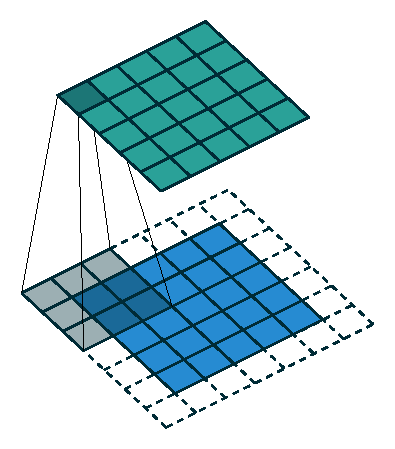
\includegraphics[width=0.23\textwidth]{figures/main/ch2-background/conv_00.pdf}
  \hfill
  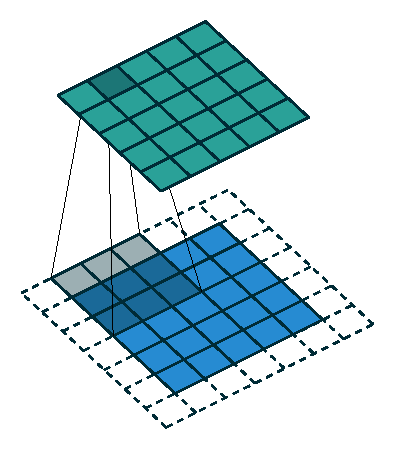
\includegraphics[width=0.23\textwidth]{figures/main/ch2-background/conv_01.pdf}
  \hfill
  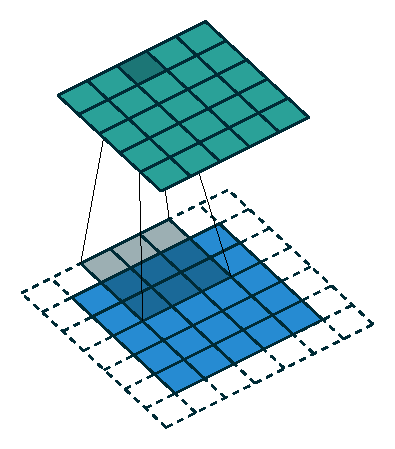
\includegraphics[width=0.23\textwidth]{figures/main/ch2-background/conv_02.pdf}
  \hfill
  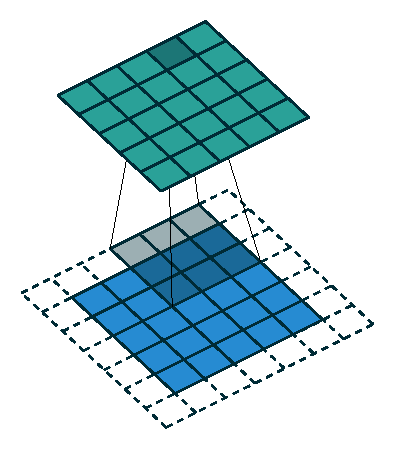
\includegraphics[width=0.23\textwidth]{figures/main/ch2-background/conv_03.pdf}
  \caption{A convolution: a kernel sliding over an image and acting as a filter. \\Illustration taken from~\citet{dumoulin2016guide}.}
  \label{figure:illustration_convolution}
\end{figure}

Doubly-block circulant and doubly-block Toeplitz matrices are very interesting structured due to their relation to 2-dimensional convolutions.
Recall that a discrete convolution can be seen as a kernel sliding over the image and acting as a filter.
\Cref{figure:illustration_convolution} illustrates the convolution operation with the image (blue), the kernel (gray) and the resulting operation (green).
It has been shown by~\citet{jain1989fundamentals} that the convolution operation is a linear transform `performed' by a doubly-block Toeplitz matrix (in the 2d case), \ie, a block Toeplitz matrix where the blocks are also Toeplitz.
Considering convolutions as a simple linear transform with a structured matrix has allowed multiple results to be derived~\citet{appuswamy2016structured,wang2020orthogonal,sedghi2018singular,singla2019bounding}, including one of our main contributions presented in \Cref{chapter:ch5-lipschitz_bound}.



% This observation has been made by~\citet{jain1989fundamentals} and many works have been derived from it~\citet{appuswamy2016structured,wang2020orthogonal,sedghi2018singular,singla2019bounding}, including one of our main contributions presented in \Cref{chapter:ch5-lipschitz_bound}.

A discrete convolution operation with a 2-dimensional kernel applied on a 2-dimensional signal is equivalent to a matrix multiplication with a doubly-block Toeplitz matrix.
Let $\Kmat$ be a 2-dimensional kernel defined as follows:
\begin{equation*}
  \Kmat = \leftmatrix
    k_0 & k_1 & k_2 \\
    k_3 & k_4 & k_5 \\
    k_6 & k_7 & k_8 
  \rightmatrix
\end{equation*}
then, the doubly-block Toeplitz matrix $\Mmat$ that performs the convolution can be represented as:
\begin{equation*}
  \Mmat = \leftmatrix
    \Tmatsf^{(0)} & \Tmatsf^{(1)} &             &  0          \\
    \Tmatsf^{(2)} & \Tmatsf^{(0)} & \ddots      &             \\
                  & \ddots        & \Tmatsf^{(0)} & \Tmatsf^{(1)} \\
    0             &               & \Tmatsf^{(2)} & \Tmatsf^{(0)}
  \rightmatrix
\end{equation*}
where $\Tmatsf^{(j)}$ are Toeplitz matrices and the values of the kernel $\Kmat$ are distributed in the Toeplitz blocks as follows:

\begin{equation*}
  \Tmatsf^{(0)} = \leftmatrix
    k_4 & k_3 &         &         & 0       \\
    k_5 & k_4 & k_3 &         &         \\
            & k_5 & \ddots  & \ddots  &         \\
            &         & \ddots  & k_4 & k_3 \\
    0       &         &         & k_5 & k_4
  \rightmatrix \quad \quad
  \hfill
  \Tmatsf^{(1)} = \leftmatrix
    k_7 & k_6 &         &         & 0       \\
    k_8 & k_7 & k_6 &         &         \\
            & k_8 & \ddots  & \ddots  &         \\
            &         & \ddots  & k_7 & k_6 \\
    0       &         &         & k_8 & k_7 \\
  \rightmatrix \quad
\end{equation*}

\begin{equation*}
  \Tmatsf^{(2)} = \leftmatrix
    k_1 & k_0 &         &         & 0       \\
    k_2 & k_1 & k_0 &         &         \\
            & k_2 & \ddots  & \ddots  &         \\
            &         & \ddots  & k_1 & k_0 \\
    0       &         &         & k_2 & k_1 \\
  \rightmatrix
\end{equation*}


However, in practice, the signal can have multiple channels (\eg, images have 3 channels: RGB).
% corresponding to the colors red, green and blue).
Let us denote by $\cin$ and $\cout$ the number of channels of the input and output respectively.
Then the convolution takes an input of size $\cin \times n \times n$, performed by a kernel of size $\cout \times \cin \times k \times k$, and outputs a signal of size $\cout \times m \times m$ with $m = n - k + 2p + 1$ where $p$ corresponds to the padding.
The matrix for the multi-channel convolution is the concatenation of $\cout \cdot \cin$ doubly-block Toeplitz matrices.





%%%%%%%%%%%%%%%%%%%%%%%%%%%%%%%%%%%%%%%%%%%%%%%%%%%%%%%%%%%%%%%%%%%%%%%%%%%%%%%
\subsection{LDR: General Framework for Structured Matrices}
\label{subsection:ch2-general_frameworks_for_structured_matrices}
%%%%%%%%%%%%%%%%%%%%%%%%%%%%%%%%%%%%%%%%%%%%%%%%%%%%%%%%%%%%%%%%%%%%%%%%%%%%%%%


Other structured matrices can benefit from reduced memory footprint and fast matrix-vector product.
Bellow a description of some known structured matrices: 
\begin{itemize}
  \item \textbf{Hankel matrix}: A Hankel matrix, named after Hermann Hankel, has constant values along each of its anti-diagonals.
  \item \textbf{Vandermonde matrix}: A Vandermonde matrix, named after Alexandre-Théophile Vandermonde, is a matrix where each term follows a geometric progression.
    A very important special case is the complex matrix associated with the Discrete Fourier transform (DFT) presented in \Cref{definition:ch2-fourier_matrix} which has a Vandermonde structure.
  \item \textbf{Cauchy matrix}: A Cauchy matrix, named after Augustin Louis Cauchy, is an $m \times n$ matrix with elements $a_{ij}$ such that $a_{ij} = (\uvec_i - \vvec_j)^{-1}$ with $\uvec_i - \vvec_j \neq 0$, $i \in \{0,\dots,m-1\}$ and $j \in \{0,\dots,n-1\}$.
\end{itemize}
\Cref{figure:ch2-example_structure_matrices} shows the representation of the parameters sharing of Hankel, Vandermonde and Cauchy matrices.
These matrices with matrices from the Toeplitz family can be unified thanks to the notion of \emph{Low Displacement Rank} (LDR).
Although these matrices appear to have very different kinds of parameter sharing, they can be all associated with a specific displacement operator $\triangleopdown_{\Amat, \Bmat}: \Rbb^{m \times n} \rightarrow \Rbb^{m \times n}$ which takes a matrix, $\Mmat$, and outputs a low rank matrix $\triangleopdown_{\Amat, \Bmat}(\Mmat)$ such that $\rank(\triangleopdown_{\Amat, \Bmat}(\Mmat)) \ll \min(m,n)$.


\begin{figure}[t]
   \centering
   \begin{subfigure}[b]{0.32\textwidth}
       \centering
       \begin{equation*}
	  \leftmatrix
	     \hvec_{n-1} & \cdots     & \hvec_1 & \hvec_0      \\
	     \vdots      & \ddots     & \hvec_0 & \hvec_{-1}   \\
	     \hvec_1     & \ddots     & \ddots  & \vdots       \\
	     \hvec_0     & \hvec_{-1} & \cdots  & \hvec_{-n+1} \\
	  \rightmatrix
       \end{equation*}
       \caption*{Hankel}
   \end{subfigure}
   \hfill
   \begin{subfigure}[b]{0.32\textwidth}
       \centering
       \begin{equation*}
	  \leftmatrix
	    1 & \vvec_0     & \cdots & \vvec_0^{n-1} \\
	    1 & \vvec_1     & \cdots & \vvec_1^{n-1} \\
	    1 & \vdots      &        & \vdots        \\
	    1 & \vvec_{n-1} & \cdots & \vvec_{n-1}^{n-1}
	  \rightmatrix
       \end{equation*}
       \caption*{Vandermonde}
   \end{subfigure}
   \hfill
   \begin{subfigure}[b]{0.32\textwidth}
       \centering
       \begin{equation*}
	  \leftmatrix
	  \frac{1}{\uvec_0 - \vvec_{0}}     & \cdots & \frac{1}{\uvec_0 - \vvec_{n-1}} \\
	  \frac{1}{\uvec_1 - \vvec_{0}}     & \cdots & \frac{1}{\uvec_1 - \vvec_{n-1}} \\
	  \vdots                            & \cdots & \vdots                          \\
	  \frac{1}{\uvec_{n-1} - \vvec_{0}} & \cdots & \frac{1}{\uvec_{n-1} - \vvec_{n-1}}
	  \rightmatrix
       \end{equation*}
       \caption*{Cauchy}
   \end{subfigure}
   \caption{Representation of Hankel, Vandermonde and Cauchy matrices}
  \label{figure:ch2-example_structure_matrices}
\end{figure}


This displacement rank approach has been initially proposed by~\citet{kailath1979displacement} and has been further studied by~\citet{kailath1995displacement,pan2001structured}.
More formally, we can define two displacement operators (for simplification, we consider $m = n$):
\begin{definition}[\emph{Sylvester} \& \emph{Stein} displacement operators]
  Let $\Amat, \Bmat \in \Rbb^{n \times n}$, the \emph{Sylvester} displacement operator denoted $\triangleopdown_{\Amat, \Bmat} = \triangleopdown_{\Amat, \Bmat}: \Rbb^{n \times n} \rightarrow \Rbb^{n \times n}$ is defined as follows:
  \begin{equation}
    \triangleopdown_{\Amat, \Bmat} (\Mmat) \triangleq \Amat \Mmat - \Mmat \Bmat
  \end{equation}
  The \emph{Stein} displacement operator denoted $\triangleopup_{\Amat, \Bmat} = \triangleopup_{\Amat, \Bmat}: \Rbb^{n \times n} \rightarrow \Rbb^{n \times n}$ is defined as follows:
  \begin{equation}
    \triangleopup_{\Amat, \Bmat} (\Mmat) \triangleq \Mmat - \Amat \Mmat \Bmat
  \end{equation}
  where $\triangleopdown_{\Amat, \Bmat} = \Amat \triangleopup_{\Amat^{-1}, \Bmat}$ if the operator matrix $\Amat$ is non-singular, and $\triangleopdown_{\Amat, \Bmat} = -\triangleopup_{\Amat, \Bmat^{-1}}$ if the operator matrix $\Bmat$ is non-singular.
\end{definition}



\begin{table}[t]
  \centering
  \begin{tabular}{c|c|c|c}
    \toprule
    \multicolumn{2}{c|}{\textbf{Operator Matrices}} & \textbf{Class of structured} & \textbf{Rank of } \\
    \textbf{A} & \textbf{B} & \textbf{matrices M} & $\triangleopdown_{\Amat, \Bmat}(\Mmat)$ \\
    \midrule
    $\Zmat_1$                & $\Zmat_{-1}$             & Toeplitz               & $\leq 2$ \\
    $\Zmat_1$                & $\Zmat_0^\top$           & Hankel                 & $\leq 2$ \\
    $\Zmat_0 + \Zmat_0^\top$ & $\Zmat_0 + \Zmat_0^\top$ & Toeplitz + Hankel      & $\leq 4$ \\
    $\diag(\vvec)$           & $\Zmat_0$                & Vandermonde            & $\leq 1$ \\
    $\Zmat_0$                & $\diag(\vvec)$           & Inverse of Vandermonde & $\leq 1$ \\
    $\diag(\uvec)$           & $\diag(\vvec)$           & Cauchy                 & $\leq 1$ \\
    $\diag(\vvec)$           & $\diag(\uvec)$           & Inverse of Cauchy      & $\leq 1$ \\
    \bottomrule
  \end{tabular}
  \caption{Displacing Matrices Associated with Families of Structured Matrices.}
  \label{table:ch2-displacing_matrices}
\end{table}



\noindent
Based on this definition, if $\Mmat$ is a structured matrix, there exist operator matrices $\Amat$ and $\Bmat$ such that $\triangleopdown_{\Amat, \Bmat} (\Mmat)$ is low rank.
In particular, $\Amat$ and $\Bmat$ can be chosen to be diagonal or $f$-unit-circulant matrices (see \Cref{definition:ch2-f_circulant_matrix}) for several classes of structured matrices.
\Cref{table:ch2-displacing_matrices} shows some specific choices of operators for the four basic classes of structured matrices and for some related matrices.
We now define the matrices that can be considered structured with respect to the Sylvester or Stein operator.
\begin{definition}[L-like matrices]
  For an $n \times n$ matrix $\Mmat$ and an associated operator $\triangleopdown_{\Amat, \Bmat}$ (or $\triangleopup_{\Amat, \Bmat}$), the value $r = \rank(\triangleopdown_{\Amat, \Bmat}(\Mmat))$ (or $r = \rank(\triangleopup_{\Amat, \Bmat}(\Mmat))$) is called the \emph{displacement rank}.
    If the value of $r$ is small relative to $n$ as $n$ grows large, then we call the matrix $\Mmat$ \emph{L-like} having a structure of type $L$.
    For example, in the case where the operator $\triangleopdown_{\Amat, \Bmat}$ is associated with Toeplitz matrices (\ie, $\Amat = \Zmat_1$ and $\Bmat = \Zmat_{-1}$, see~\Cref{table:ch2-displacing_matrices}), we call the matrix $\Mmat$, \emph{Toeplitz-Like}.
  \label{definition:ch2-l_like_matrices}
\end{definition}

An important result allows us to express structured matrices with low-displacement rank directly as a function of its low displacement generators.
For the Stein type displacement operator, the following result holds:
\begin{theorem}[Krylov Decomposition~\citet{pan2003inversion,sindhwani2015structured}] \label{theorem:ch2-krylov_decomposition}
  If an $n \times n$ matrix $\Mmat$ is such that $\triangleopup_{\Amat, \Bmat}(\Mmat) = \Gmat \Hmat^\top$ where 
  $\Gmat = (\gvec^{(1)} \ldots \gvec^{(r)}), \Hmat = (\hvec^{(1)} \ldots \hvec^{(r)}) \in \Rbb^{n \times r}$ 
  and the operator matrices satisfy: $\Amat^n = a \Imat$, $\Bmat^n = b \Imat$ for some scalars $a, b$, then $\Mmat$ can be expressed as: 
  \begin{equation} \label{equation:ch2-krylov_decomposition}
    \Mmat = \frac{1}{1 - ab} \sum_{j=1}^{r} ~\krylov(\Amat, \gvec^{(j)}) ~\krylov(\Bmat^\top, \hvec^{(j)})^\top
  \end{equation}
  where $\krylov(\Amat, \vvec)$ is defined by:
  \begin{equation}
    \krylov(\Amat, \vvec) = [\vvec~~\Amat\vvec~~\Amat^2 \vvec~~\ldots~~\Amat^{n-1} \vvec]
  \end{equation}
  \removespace
\end{theorem}

\noindent
This theorem can be used to decompose structured matrices and define efficient algorithms for matrix-vector products.
For example, this theorem can be simplified for \emph{Toeplitz-like matrices} as follows:
\begin{theorem}[Toeplitz-like matrix decomposition \citet{pan2001structured}] \label{theorem:ch2-toeplitz_like}
  If an $n \times n$ matrix $\Mmat$ satisfies $\triangleopdown_{\Zmat_1, \Zmat_{-1}}(\Mmat) = \Gmat \Hmat^\top$ $(\Mmat \text{ is Toeplitz-like})$ where $\Gmat = (\gvec ^{(1)} \ldots \gvec^{(r)}), \Hmat = (\hvec^{(1)} \ldots \hvec^{(r)}) \in \Rbb^{n \times r}$, then $\Mmat$ can be written as: 
  \begin{equation} \label{equation:ch2-toeplitz_like_matrix_decomposition}
    \Mmat = \sum_{j=1}^{r} \Zmat_1(\gvec^{(j)}) \Zmat_{-1}(\Jmat_n \hvec^{(j)})
  \end{equation}
  where $\Jmat_n$ is the reflection matrix of size $n \times n$ (reflection of the identity matrix such that $\Jmat^2 = \Imat$) and $\Zmat_1$ and $\Zmat_{-1}$ are $f$-unit-circulant matrices (see \Cref{definition:ch2-f_circulant_matrix}).
\end{theorem}
\noindent
In the next chapter, we will see how this general framework have been used in the context of compact neural networks.





%%%%%%%%%%%%%%%%%%%%%%%%%%%%%%%%%%%%%%%%%%%%%%%%%%%%%%%%%%%%%%%%%%%%%%%%%%%%%%%
\section{Supervised Learning and Neural Networks}
\label{section:ch2-supervised_learning_neural_networks}
%%%%%%%%%%%%%%%%%%%%%%%%%%%%%%%%%%%%%%%%%%%%%%%%%%%%%%%%%%%%%%%%%%%%%%%%%%%%%%%
%%%%%%%%%%%%%%%%%%%%%%%%%%%%%%%%%%%%%%%%%%%%%%%%%%%%%%%%%%%%%%%%%%%%%%%%%%%%%%%
\subsection{Introduction to Supervised Learning}
\label{subsection:ch2-introduction_on_supervised_learning}
%%%%%%%%%%%%%%%%%%%%%%%%%%%%%%%%%%%%%%%%%%%%%%%%%%%%%%%%%%%%%%%%%%%%%%%%%%%%%%%

Supervised learning consists in learning a function that maps an input to an output based on input-output pairs.
For example, one could learn to ``predict'' if a fruit will be tasty based on its features (\eg size, weight, color, consistency, etc.).
These features are used as inputs to the function and the function outputs a value characterizing the taste of the fruit. 

In the following, we will formalize the learning problem described above with the \emph{statistical learning framework}.
First, let us define the domain space $\Xset$ which corresponds to the set of inputs that we wish to label.
Let us denote the label space $\Yset$ and a finite sequence of pairs $\mathcal{S} = \left\{ \left(\xvec^{(1)}, y^{(1)} \right) \dots \left( \xvec^{(m)}, y^{(m)} \right) \right\}$ in $\Xset \times \Yset$. 
Such pairs \ie, labeled examples, are called \emph{training examples} and the set $\mathcal{S}$ is called the \emph{training set}.
We denote $\mathcal{D}$ the \emph{joint distribution} over $\Xset \times \Yset$.
The main objective of the task at hand is to output a \emph{prediction rule} $h: \Xset \rightarrow \Yset$ that maps the input $\xvec \in \Xset$ to the output $y \in \Yset$.
This function is called the \emph{hypothesis} or the \emph{classifier}. 
Given the probability distribution $\mathcal{D}$, we aim to measure how \emph{likely} the hypothesis $h$ makes an error when labeled points are randomly drawn from the distribution $\mathcal{D}$.
Let us define the true error or \emph{risk} of the hypothesis $h$ that we wish to minimize:
% \begin{equation}
%   R_{\mathcal{D}}(h) \triangleq \Pbb_{(\xvec, y) \sim \mathcal{D}} \left[ h(\xvec) \neq  y \right] \enspace.
%   \label{equation:ch2-risk1}
% \end{equation}
\begin{equation} \label{equation:ch2-risk2}
  R_{\mathcal{D}}(h) \triangleq \Ebb_{(\xvec, y) \sim \mathcal{D}} \left[ L\big( h(\xvec), y \big) \right] \enspace.
\end{equation}
where $L: \Yset \times \Yset \rightarrow \Rbb_{+}$ is a \emph{loss function} which measures the correctness of the hypothesis.
For example, for classification problems, we can define $L$ as: %$L(h(\xvec), y) = \mathds{1}_\big[ h(\xvec) \neq y \big]$.
\begin{equation}
  L(h(\xvec), y) = \mathds{1}_{\big[ h(\xvec) \neq y \big]}
\end{equation}

However, in practice, the joint probability distribution $\mathcal{D}$ is unknown; therefore, the true error is not directly available to the learner.
The learner only has access to the training data, $\mathcal{S}$, and can calculate the \emph{empirical error} \ie, the error over the training samples.
We define the \emph{empirical risk} as follows:
\begin{equation}
  R_{\mathcal{S}}(h) \triangleq \frac{1}{|\mathcal{S}|} \sum_{(\xvec, y) \in \mathcal{S}} L\big( h(\xvec), y \big) \enspace.
\end{equation}


% \begin{equation}
%   R_{\mathcal{S}}(h) \triangleq \frac{\left| \left\{i \in [m]: h\left(\xvec^{(i)}\right) \neq y^{(i)} \right\}\right|}{m} \enspace.
% \end{equation}
% We can generalize our measure of correctness so that it can be applied to multiple learning tasks.
% Let us define a \emph{loss function} from $\Yset \times \Yset$ to the set of nonnegative real numbers, $L: \Yset \times \Yset \rightarrow \Rbb_{+}$.
% We can express the \emph{risk} as follows:
% \begin{equation}
%   R_{\mathcal{D}}(h) \triangleq \Ebb_{(\xvec, y) \sim \mathcal{D}} \left[ L\big( h(\xvec), y \big) \right] \enspace.
%   \label{equation:ch2-risk2}
% \end{equation}
% Similarly, we express the empirical risk as follows:
% \begin{equation}
%   R_{\mathcal{S}}(h) \triangleq \frac{1}{m} \sum_{(\xvec, y) \sim \mathcal{S}} L\big( h(\xvec), y \big) \enspace.
% \end{equation}
% The loss functions used for classification problems and regression problems are as follows: 
% \begin{itemize}
%   \item \textbf{0-1 Loss}: $L_{0-1}\big( h(\xvec), y \big) = \mathds{1}_\big[ h(\xvec) \neq y \big]$ \\
%   This loss is used for classification problems, for example, when the learner have to recognizing hand-written digits in images.
%   We can notice that the definitions of $R_{\mathcal{D}}$ given in \Cref{equation:ch2-risk1} and \Cref{equation:ch2-risk2} coincide.
%   \item \textbf{Square Loss}: $L_{\text{sq}} \big( h(\xvec), y \big) = \big( h(\xvec) - y \big)^2$ \\	
%   This loss is used for another common type of learning problem \ie, \emph{regression problem}, in which the label domain $\Yset$ is the set of real numbers.
%   For example, one wishes to predict the price of an apartment given its characteristics.
% \end{itemize}


The goal of the learning algorithm is to find the hypothesis $h$ that minimizes the risk $R_{\mathcal{S}}$, this learning paradigm is called \emph{Empirical Risk Minimization} (ERM).
We use the ERM paradigm as a surrogate to find a hypothesis $h$ that minimizes the true risk $R_\mathcal{D}$.
However, all hypotheses that minimize the empirical error do not necessarily minimize the true risk.
For example, consider the following function:
\begin{equation} \label{equation:ch2-perfect_function}
  h^*(\xvec) =
  \begin{cases}
    y^{(i)} &\quad \text{if }\exists i \in [m] \text{ s.t. } \xvec^{(i)} = \xvec \\
    0 &\quad \text{otherwise}
  \end{cases}
\end{equation}
Clearly, this function, for any training set, $\mathcal{S}$, will have $R_\mathcal{S}(h^*) = 0$, whereas the true risk would certainly be high.
The phenomenon, called \emph{overfitting}, happens when the classifier fits the training data ``too well'' but will likely have a high error on unseen data.
One possible solution to this phenomenon is to apply ERM with a restricted search space to prevent the learning algorithm to output a function such as $h^*$ in \Cref{equation:ch2-perfect_function}.
We call this set the \emph{hypothesis class} and is denoted $\mathcal{H}$.
Each $h \in \mathcal{H}$ is a function mapping from $\Xset$ to $\Yset$.
We call $\mathrm{ERM}_{\mathcal{H}}$, the set of learned hypotheses that uses the $\mathrm{ERM}$ paradigm over the hypothesis class $\mathcal{H}$ and a training data $\mathcal{S}$.
Formally,
\begin{equation}
  \mathrm{ERM}_{\mathcal{H}}(\mathcal{S}) \in \argmin_{h \in \mathcal{H}} R_{\mathcal{S}}(h) \enspace.
\end{equation}
For a training sample $\mathcal{S}$, we denote $h_\mathcal{S}$, one solution of applying $\text{ERM}_\mathcal{H}$ on the set $\mathcal{S}$, if there exists multiple hypotheses with minimal error on the training sample, then the minimization problem returns an arbitrary one.
In practice, the hypothesis class is chosen based on a hypothesis on the relation between the data and its label.
For example, if the relation between the data and its label is supposedly linear then the hypothesis class can be the set of all linear functions.
This kind of restriction is called an \emph{inductive bias} because the learner is \emph{biased} toward a particular set of predictors.

\begin{figure}[t]
  \centering
  \begin{subfigure}[b]{0.32\textwidth}
    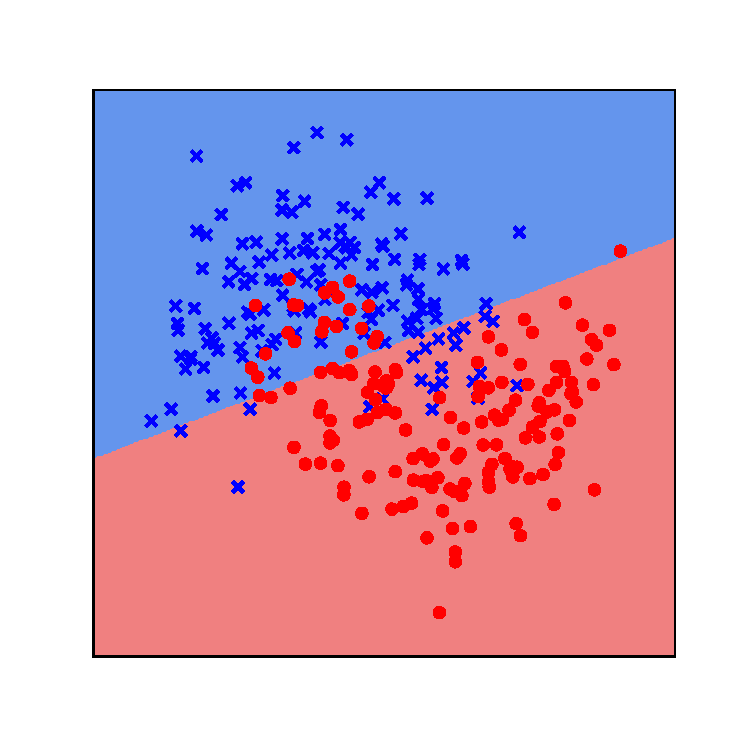
\includegraphics[width=0.98\textwidth]{figures/main/ch2-background/underfitting.pdf}
    \caption{Underfitting}
    \label{figure:ch2-fitting_points_a}
  \end{subfigure}
  \hfill
  \begin{subfigure}[b]{0.32\textwidth}
    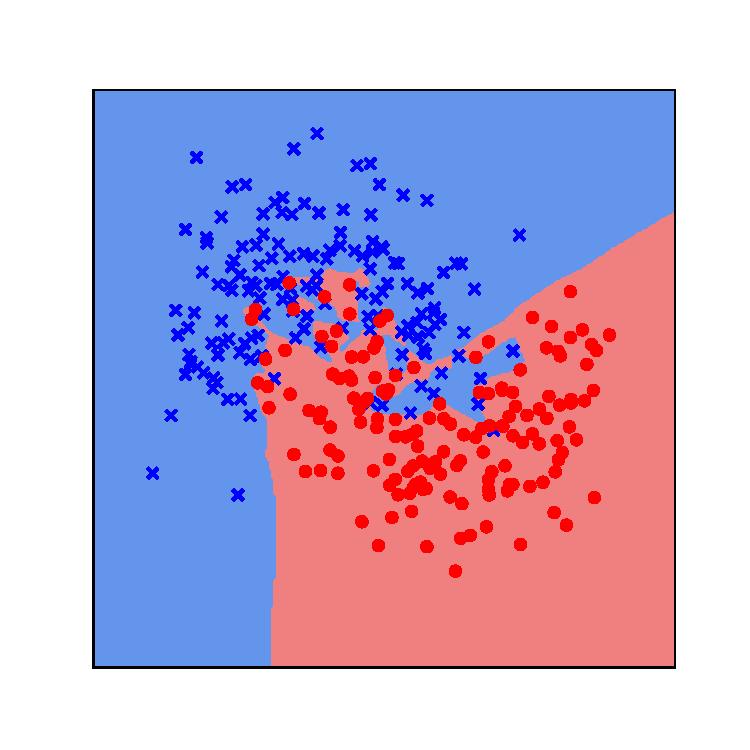
\includegraphics[width=0.98\textwidth]{figures/main/ch2-background/overfitting.pdf}
    \caption{Overfitting}
    \label{figure:ch2-fitting_points_b}
  \end{subfigure}
  \hfill
  \begin{subfigure}[b]{0.32\textwidth}
    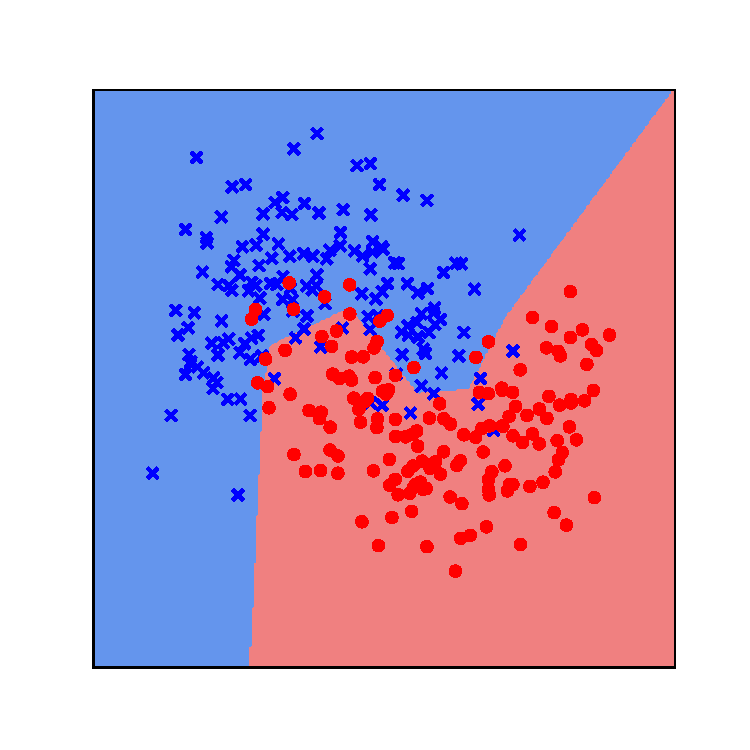
\includegraphics[width=0.98\textwidth]{figures/main/ch2-background/normal.pdf}
    \caption{Good fit}
    \label{figure:ch2-fitting_points_c}
  \end{subfigure}
  \caption{
    Decision boundary of 3 classifiers with different complexity for the same set of samples.
  }
  \label{figure:ch2-fitting_points}
\end{figure}



A fundamental question remains: \emph{how to choose the correct hypothesis class for which $\text{ERM}_\mathcal{H}$ will not lead to overfitting?} 
We answer this question by decomposing the true risk into two different components as follows: 
\begin{equation} \label{equation:ch2-bias_complexity_tradeoff}
  R_\mathcal{D} (h_\mathcal{S}) = 
  \underbrace{\left[ \min_{h \in \mathcal{H}} R_\mathcal{D}(h) \right]}_{\text{\scriptsize Approximation Error}} + \quad 
  \underbrace{\left[ R_\mathcal{D}(h_\mathcal{S}) - \min_{h \in \mathcal{H}} R_\mathcal{D}(h) \right]}_{\text{\scriptsize Estimation Error}} 
\end{equation}
\begin{itemize}
  \item \textbf{Approximation Error}: The approximation error corresponds to the minimum risk achievable by a classifier in the given hypothesis class.
  Intuitively, this error measures the quality of the hypothesis class and therefore the quality of the prior knowledge.
  Enlarging the hypothesis class, \ie, allowing more complex functions, can decrease the approximation error.
  \item \textbf{Estimation Error}: The estimation error is the difference between the approximation error and the error made by the ERM predictor.
  Recall that the empirical risk is only an estimate of the true risk.
  This error is dependent on the sample size and/or the complexity of the hypothesis class. 
\end{itemize}
Recall that the main goal is to minimize the true risk $R_\mathcal{D} (h_\mathcal{S})$, however, \Cref{equation:ch2-bias_complexity_tradeoff} shows a tradeoff called the \emph{bias-complexity tradeoff}.
The tradeoff is as follows: if we choose a large and complex hypothesis space, we reduce the approximation error but at the same time we can increase the estimation error because a complex hypothesis space might lead to overfitting.
Conversely, choosing a small hypothesis space might reduce the estimation error but increase the approximation error leading to an \emph{underfitting} phenomenon.
We can illustrate the \emph{overfitting} and \emph{underfitting} phenomenons with \Cref{figure:ch2-fitting_points} which shows the decision boundary of 3 classifiers for the same set of samples.
\Cref{figure:ch2-fitting_points_a} shows a classifier which \emph{underfit} the data, meaning the decision boundary is not complex enough to separate the data correctly.
\Cref{figure:ch2-fitting_points_b} shows a classifier that almost perfectly follows the training data but is likely to have a higher error rate on the unseen data.
Finally, \Cref{figure:ch2-fitting_points_c} shows a classifier that seems to have a good compromise between the two.


As seen above, defining a small hypothesis class might lead to underfitting and a large hypothesis class might lead to overfitting.
A good way to best balance the trade-off would be to minimize the empirical risk while also minimizing the complexity of the hypothesis class. 
Let us define a \emph{regularization} function $r: \mathcal{H} \rightarrow \Rbb$ which takes an hypothesis as input and a measure of the ``complexity'' of the hypothesis.
We could now update the learning rule as follows:
\begin{equation}
  \argmin_{h \in \mathcal{H}} \left[ R_\mathcal{S}(h) + r(h) \right]
\end{equation}
This learning rule minimizes the empirical risk $R_\mathcal{S}(h)$ and the regularization function $r$, thus, preventing overfitting and improving generalization on unseen data.
This learning rule is closely related to \emph{Structural Minimization Paradigm} (SRM) \cite{shalev2014understanding}.
In the next section, we will present a classical regularization function for neural networks and we will introduce a new regularization scheme in \Cref{chapter:ch5-lipschitz_bound}.




% A good way to offset a large hypothesis class would be to specific preference over hypothesis within the hypothesis class.
% The \emph{Structural Minimization Paradigm} (SRM) assumes that the hypothesis class can be written as the union of multitude smaller hypothesis class as follows: $\mathcal{H} = \bigcup_{n \in \Nbb} \mathcal{H}_n$ with a weight function $w: \Nbb \rightarrow [0, 1]$ which assigns a weight to each hypothesis class, $\mathcal{H}_n$, such that a higher weights reflects a lower preference for the hypothesis class.
% Intuitively, the weight function is a measure of the ``complexity'' of the hypotesis.
% The SRM learning paradigm can then be defined as follows:
% \begin{equation}
%   \text{SRM}_\mathcal{H} \in \argmin_{h \in \mathcal{H}, n \in \Nbb} \left[ R_\mathcal{S}(h) + w(n) \right]
% \end{equation}
% The SRM learning paradigm minimizes the empirical risk $R_\mathcal{S}(h)$ and the weight function $w$; therefore, ovoiding overfitting and improving generalization by reducing the complexity of the hypotesis while maintening a low empirical risk. 
% In the next section, we will present neural networks which are the type of function we will use as predictors and we will see how to implement the ERM and SRM paradigm.









% \‰\‰\‰
%
% The ERM paradigm with inductive bias is based on an important assumption.
% We assume that uniformly over all $h \in \mathcal{H}$, the empirical risk is close to the true risk, meaning, an $h$ that minimize the empirical risk with respect to a data set $\mathcal{S}$ will also minimize the \emph{true} risk.
% More formally, 
% \begin{equation}
%   \forall h \in \mathcal{H}, \quad \left| R_\mathcal{S}(h) - R_\mathcal{D}(h) \right| \leq \epsilon \enspace.
%   \label{equation:ch2-eps_respresentative_sample} 
% \end{equation}
% If this assumption is met, then the ERM paradigm will always return a good classifier. 
% \begin{lemma}[Lemma 4.2 \citet{shalev2014understanding}] 
%   If \Cref{equation:ch2-eps_respresentative_sample} hold, then any output of $\mathrm{ERM}_\mathcal{H}(\mathcal{S})$, namely, any $h_\mathcal{S} \in \argmin_{h \in \mathcal{H}} R_\mathcal{S}(h)$, satisfies
%   \begin{equation}
%     R_\mathcal{D}(h_\mathcal{S}) \leq \min_{h \in \mathcal{H}} R_\mathcal{S}(h) + 2\epsilon
%   \end{equation}
% \end{lemma}
%
% \‰\‰\‰


% Let us consider an input space $\Xset = [0, 1]^d$ of dimension $d$, an output space $\Yset = [k]$ where $k$ is the number of class and a data distribution $\mathcal{D}$ over $\Xset \times \Yset$.
% We seek to find a function $h: \Xset \rightarrow \Yset$ that maps the input $\xvec \in \Xset$ to the output $y \in \Yset$ with $h \in \mathcal{H}$ where $h$ is called the \emph{hypothesis} and $\mathcal{H}$ the \emph{hypothesis space}.
% in order to measure how well the function fits, we de\emph{loss function} $l: \mathcal{y} \times \mathcal{y} \rightarrow \rbb^{+}$ is defined.
% The \emph{risk} $R$ associated with the hypothesis $h(\xvec)$ is defined as follows:
% \begin{equation}
%   R(h) \triangleq \Ebb_{(\xvec, y) \sim \mathcal{D}}\  L \left( h(\xvec), y \right)
% \end{equation}
% The goal of a \emph{learning algorithm} is to find a hypothesis $h^* \in \mathcal{H}$ which minimize the risk $R(h)$:
% \begin{equation}
%   h^* \triangleq \argmin_{h \in \mathcal{H}} R(h) .
% \end{equation}

% In practice, the joint probability distribution $\mathcal{D}$ is unknown.
% Instead, we have $n$ independent observations of the distribution called the \emph{training set}
% \begin{equation}
%   \mathcal{T} \triangleq \left\{ \left(\xvec^{(1)}, y^{(1)} \right), \dots, \left( \xvec^{(n)}, y^{(n)} \right) \right\} ,
% \end{equation}
% where $\xvec \in \Xset$ and $y \in \Yset$.

% The risk minimization problem is therefore replace by the \emph{empirical risk minimization} as follows:
% \begin{equation}
%   E(h, n) \triangleq \frac{1}{n} \sum_{i = 1}^{n} L\left(h\left(\xvec^{(i)}\right), y^{(i)}\right) ,
% \end{equation}
% the learning algorithm then becomes:
% \begin{equation}
%   \hat{h}^* \triangleq \argmin_{h \in \mathcal{H}} E(h, n)  .
% \end{equation}


% \paragraph{Structural Risk Minimization} (SRM).
% The ERM principle assumes that the function $\hat{h}^*$ minimizing $E(h, n)$ leads to the risk $R(\hat{h}^*)$ being close to the minimum.
% This assumption mean that as the \emph{size} of the training set increase the minimization becomes more accurate. More formally, the ERM principle assumes that $R(\hat{h}^*)$ converge to its minimum value on the set $h \in \mathcal{H}$ when $n \rightarrow \infty$.  
% \citet{Vapnik1991TheNA} have shown that this equivalent to say that the empirical risk $E(h, n)$ \emph{converge uniformly} to the actual risk $R(h)$ over $h \in \mathcal{H}$ where the \emph{uniform convergence} is defined as follows:
% \begin{equation}
%   \Pbb \left[ \sup_{h \in \mathcal{H}} \left| R(h) - E(h, n) \right| < \epsilon \right] \rightarrow 0 \quad \text{ when } \quad n \rightarrow \infty, \quad \forall \epsilon > 0 
% \end{equation}


% \citet{Vapnik1991TheNA} have shown that this assumption is equivalent to the following: does the empirical risk $E(h, n)$ \emph{converge uniformly} to the actual risk $R(h)$ over $h \in \mathcal{H}$ where the \emph{uniform convergence} is defined as follows:
% \begin{equation}
%   \Pbb \left[ \sup_{h \in \mathcal{H}} \left| R(h) - E(h, n) \right| < \epsilon \right] \rightarrow 0 \quad \text{ when } \quad n \rightarrow \infty, \quad \forall \epsilon > 0 
% \end{equation}


% However, does increasing the \emph{size} of the training set allow a better minimisation of the actual risk. More formally, does $R(\hat{h}^*)$ converge to its minimum value on the set $h \in \mathcal{H}$ when $n \rightarrow \infty$. 

% \citet{vapnik1992principles} 

% The 0-1 loss function is a natural loss function to use because it assigns 0 for a correct classification and 1 for an incorrect classification. 


% of the ERM principle \ie, does $R(\hat{h}^*)$ converge to its minimum value on the set $h \in \mathcal{H}$ when $n \rightarrow \infty$ is equivalent to the question: 

% is equivalent to the question: does the empirical risk E(h, n) \emph{converge uniformly} to the actual risk $R(h)$ over $h \in \mat

% \begin{equation}
%   h^* = \argmin_{h \in \mathcal{H}} \frac{1}{n} \sum_{i = 0}^{n} L(h(\xvec_i), y) + \lambda C(\theta) 
% \end{equation}

% Because the relation between $\xvec \in \Xset$ and $y \in \Yset$ is unknown, we aim to find the best approximation of the function $h$ with a parameterized function $h_\theta \in \mathcal{H}$ where $\mathcal{H}$ is called the \emph{hypothesis space}.

% The goal of a \textbf{learning algorithm} is to learn a function $f: \Xset \rightarrow \Yset$ which outputs $y \in \Yset$ given an input $\xvec \in \Xset$ with $f \in \mathcal{H}$ where $\mathcal{H}$ is called the \emph{hypothesis space}.

% The supervised learning settings assume that a function $f: \Xset \rightarrow \Yset$ exists. 

% The supervised learning settings assume that a function $f$ that maps $\xvec \sim \Xset$ to $y \sim \mathcal{y}$ exists. 

% The goal of a \textbf{learning algorithm} is to approximate $f$ by a parameterized function $f_\theta$.
% The standard method to learn the set of parameters $\theta$ is the \textbf{empirical risk minimization (ERM)}:
% \begin{equation*}
%   \hat{\theta}_{ERM} \triangleq \argmin_{\theta} \frac{1}{n} \sum_{i=1}^{n} L (f_{\theta} (\xvec_i), y_i )
% \end{equation*}

% \begin{equation}
%   \min_{\theta} \Ebb_{(\xvec, y) \sim \mathcal{D}} \left[ L(f_\theta(x), y) \right]. 
% \end{equation}

%%%%%%%%%%%%%%%%%%%%%%%%%%%%%%%%%%%%%%%%%%%%%%%%%%%%%%%%%%%%%%%%%%%%%%%%%%%%%%%
\subsection{Preliminaries on Neural Networks}
\label{subsection:ch2-preliminaries_on_neural_networks}
%%%%%%%%%%%%%%%%%%%%%%%%%%%%%%%%%%%%%%%%%%%%%%%%%%%%%%%%%%%%%%%%%%%%%%%%%%%%%%%


% \begin{figure}[ht]
%   \centering
%   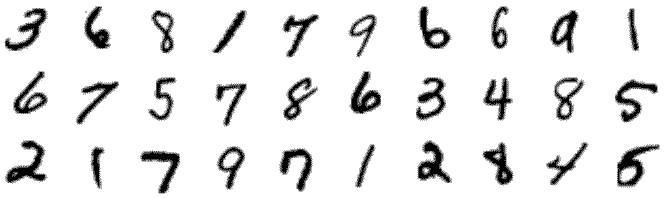
\includegraphics[width=0.88\textwidth]{figures/main/ch2-background/mnist-dataset.png}
%   \caption{Images with handwritten digits in the MNIST database \cite{lecun1998gradient}}
%   \label{figure:ch2-mnist-database}
% \end{figure}
%
% In \citeyear{lecun1998gradient}, \citeauthor{lecun1998gradient} had successfully learned a function capable of recognizing handwritten digits in images.
% They used the MNIST dataset \cite{lecun1998gradient} consisting of black and white images of size $28 \times 28$ pixels (\Cref{figure:ch2-mnist-database} presents a sample of images from the MNIST database).
% Their goal was to develop an algorithm that takes a vector as input and produces one digit from 0 to 9 as the output.
% Although simple for a human, this task is a non-trivial problem for computers due to the uniqueness of each image. 
% To solve this problem, \citet{lecun1998gradient} trained a neural network based on the images of the MNIST dataset and their labels.

% This is a non-trivial problem because each image is unique and while digits can be differentiated based on their shapes and strokes, these features give poor results for an automated system. 

% In the previous section, we said that we restrict the learner towards a specific set of predictors.
% In this thesis, we focus on neural networks. 
Neural networks, which find their roots in the work of \citet{mcculloch1943logical,rosenblatt1958perceptron}, can be analytically described as a composition of linear functions interlaced with non-linear functions (also called activation functions).
A neural network can be defined as follows:

% \begin{definition}[Neural Network]
%   Given a depth $\depth \in \Nbb$, 
%   let $w = \{ w^{(i)} \}_{i \in [\depth]}$ and $b = \{ b^{(i)} \}_{i \in [\depth]}$ be sequences of ``dimension'',  
%   $\weights = \left\{ \left( \Wmat^{(i)}, \bvec^{(i)} \right) \right\}_{i \in [\depth]}$ a set of weights matrices and bias vectors 
%   such that $\Wmat^{(i)} \in \Rbb^{w^{(i)}}$ and $\bvec^{(i)} \in \Rbb^{b^{(i)}}$ and 
%   sequence of activation functions $\act = \{\act_i \}_{i \in [\depth]}$.
% %   Let $\dim^{w} = \{ \dim_1^w, \dots, \dim_\depth^w \}$ and $\dim^{b} = \{ \dim_1^b, \dots, \dim_\depth^b \}$ 
% % be sequences of ``dimension'', let $\dim_{\text{in}} = \dim_\depth^w$ and $\dim_{\text{out}} = \dim_\depth^w$.
%   Let $\Xset \subset \Rbb^{\dim_{\text{in}}}$ and 
%   $\Yset \subset \Rbb^{\dim_\text{out}^w}$ be the input space and output space respectively. 
%   % Given a depth $\depth$, a set of weights matrices and bias vectors $\weights = \left\{ \left( \Wmat^{(i)}, \bvec^{(i)} \right) \right\}_{i \in [\depth]}$ and a sequence of activation functions $\act = \{\act_i \}_{i \in [\depth]}$, a neural network is a function $N^\act_\weights : \Xset \rightarrow \Yset$ such that
%   A neural network is a function $N^\act_\weights : \Xset \rightarrow \Yset$ such that
%   \begin{equation}
%     \nn^\act_{\weights}(\xvec) \triangleq \layer^{\act_\depth}_{\Wmat^{(\depth)}, \bvec^{(\depth)}} \circ \cdots \circ \layer^{\act_1}_{\Wmat^{(1)}, \bvec^{(1)}}(\xvec)
%   \end{equation}
%   % where $d$ corresponds to the depth of the network (\ie, the number of layers), $\weights$ is the set of weights matrices and bias vectors $\weights = \left\{ \left( \Wmat^{(1)}, \bvec^{(1)} \right) \dots \left( \Wmat^{(d)}, \bvec^{(d)} \right) \right\}$.
%   % $\Bmat$ is the set of bias vectors $\Bmat = \left\{ \right\}$. 
%   where $\layer^{\act_i}_{\Wmat^{(i)},\bvec^{(i)}}: \Rbb^{w^{(i)}} \rightarrow \Rbb^{w^{(i+1)}}$ (also called layer) is a function parameterized by the weight matrix $\Wmat^{(i)}$, the bias vector $\bvec^{(i)}$ and the activation function $\act_i$ and can be expressed as follows: 
%   \begin{equation}
%     \layer^{\act_i}_{\Wmat^{(i)},\bvec^{(i)}} (\xvec) \triangleq \act_i \left(\Wmat^{(i)}\xvec + \bvec^{(i)}\right)
%   \end{equation}
% \end{definition}

\begin{definition}[Neural Network] \label{definition:ch2-neural_networks}
  Given a depth $\depth \in \Nbb$, 
  let $\dimw = \{ \dimw^{(i)} \}_{i \in [\depth]}$ and $\dimb = \{ \dimb^{(i)} \}_{i \in [\depth]}$ be sequences of integers, $\weights = \left\{ \left( \Wmat^{(i)}, \bvec^{(i)} \right) \right\}_{i \in [\depth]}$ a set of weights matrices and bias vectors 
  such that $\Wmat^{(i)} \in \Rbb^{\dimw^{(i)}}$ and $\bvec^{(i)} \in \Rbb^{\dimb^{(i)}}$ and a sequence of activation functions $\act = \{\act_i \}_{i \in [\depth]}$.
  Let $\Xset \subset \Rbb^{\dimw^{(1)}}$ and $\Yset \subset \Rbb^{\dimw^{(\depth)}}$ be the input and output spaces respectively. 
	$\dimw^{(1)}$ and $\dimw^{(\depth)}$ refer to the input and output dimension respectively.
  % $\dimw^{(1)}$ refers to the input dimension and $\dimw^{(\depth)}$ refers to the output dimension.
  A neural network is a function $\nn^\act_\weights : \Xset \rightarrow \Yset$ such that
  \begin{equation}
    \nn^\act_{\weights}(\xvec) \triangleq \layer^{\act_\depth}_{\Wmat^{(\depth)}, \bvec^{(\depth)}} \circ \cdots \circ \layer^{\act_1}_{\Wmat^{(1)}, \bvec^{(1)}}(\xvec)
  \end{equation}
  where $\layer^{\act_i}_{\Wmat^{(i)},\bvec^{(i)}}: \Rbb^{w^{(i)}} \rightarrow \Rbb^{w^{(i+1)}}$ (also called layer) is a function parameterized by the weight matrix $\Wmat^{(i)}$, the bias vector $\bvec^{(i)}$ and the activation function $\act_i$.
  $\layer^{\act_i}_{\Wmat^{(i)},\bvec^{(i)}}:$  is defined as follows: 
  \begin{equation}
    \layer^{\act_i}_{\Wmat^{(i)},\bvec^{(i)}} (\xvec) \triangleq \act_i \left(\Wmat^{(i)}\xvec + \bvec^{(i)}\right) \enspace,
  \end{equation}
  and $\rho_\depth$ is identity function.
\end{definition}

\noindent
Based on this definition, for a given training set $\mathcal{S} = \Xset \times [k]$, a set of activation functions $\act$, a set of weights and biases $\weights$ and a loss function $L: \Yset \times [k] \rightarrow \Rbb_+$, the ERM learning paradigm for neural networks is given by
\begin{equation} \label{equation:ch2-erm_neural_network}
  \argmin_{\weights} \frac{1}{|\mathcal{S}|} \sum_{(\xvec, y) \in \mathcal{S}} L(N^\act_\weights(\xvec), y) 
\end{equation}
For classification problems, the zero-one loss is known to be non-convex and non-smooth, and it has been shown that solving for the optimal solution is an NP-hard combinatorial optimization problem~\cite{feldman2012agnostic,bendavid2003difficulty}.
Instead, a common approach is to use a surrogate such as the cross-entropy loss function and estimate the parameters by maximizing the \emph{likelihood} over the data.
The cross-entropy loss $L:\Yset \times [k]$, is defined as follows:
\begin{equation}
  L(N^\rho_\Omega(\xvec), y) = -\log
    \left(
      \frac
        {e^{\left(N^\rho_\Omega(\xvec)\right)_y}}
	{\sum_{j\in[k]} e^{\left(N^\rho_\Omega(\xvec)\right)_j}}
    \right)
\end{equation}
The generic approach for minimizing the empirical risk in \Cref{equation:ch2-erm_neural_network} is by \emph{gradient descent} with the \emph{backpropgation} algorithm ~\cite{rumelhart1986learning} which consists in computing the gradient with the chain-rule.




% Instead, a common approach is to used the softmax activation function as the last non-linear activation $\act_d$ with the cross-entropy loss function and estimate the parameters with \emph{maximum likelihood}~\cite{hastie2009elements}.
% The softmax activation function, $\act_d: \Rbb^k \rightarrow [0, 1]^k$, is defined as follows:
% \begin{equation}
%   \leftmat \act_d(\xvec) \rightmat_i = \frac{e^{\xvec_i}}{\sum_{j=0}^{k-1} e^{\xvec_j}}, \quad \forall i \in [0,k-1]
% \end{equation}
% The generic approach for minimizing the empirical risk in \Cref{equation:ch2-erm_neural_network} is by \emph{gradient descent} with the \emph{backpropgation} algorithm ~\cite{rumelhart1986learning} which consists of computing the gradient with the help of the chain-rule.


As seen in the previous section, the SRM paradigm minimizes two terms, the empirical risk and a weight function measuring the ``complexity'' of the hypothesis.
% It has been shown that the number of free parameters can be used as a measure of complexity and a number of work have proposed techniques to reduce the number parameters~\cite{lecun1990optimal,thodberg1991improving,weigend1991generalization}.
% However, a different way of constraining the complexity is to limit the growth of weights~\cite{hinton1987learning}.
% This \emph{regularization} \cite{tikhonov1977solutions,krogh1992simple}, also called \emph{weight decay}, prevents weights from growing too large unless it is necessary.
It has been shown that the $\ell_2$ norm of the weights of a network can be used as a measure of complexity; therefore, limiting the growth of the weights constrains the complexity of the network ~\cite{hinton1987learning}.
% However, a different way of constraining the complexity is to limit the growth of weights~\cite{hinton1987learning}.
This \emph{regularization} \cite{tikhonov1977solutions,krogh1992simple}, also called \emph{weight decay}, prevents weights from growing too large unless it is necessary.
The SRM learning algorithm with the weight decay regularization can be expressed as follows:
\begin{equation}
  \argmin_{\weights} \frac{1}{|\mathcal{S}|} \sum_{(\xvec, y) \in \mathcal{S}} L(N^\act_\weights(\xvec), y) + \lambda \sum_{(\Wmat, \bvec) \in \weights} \left( \norm{\Wmat}_\mathrm{F} + \norm{\bvec}_\mathrm{2} \right)
\end{equation}
where $\lambda > 0$ is the regularization parameter.


\begin{figure}[htb]
  \centering
  \begin{subfigure}[b]{0.32\textwidth}
    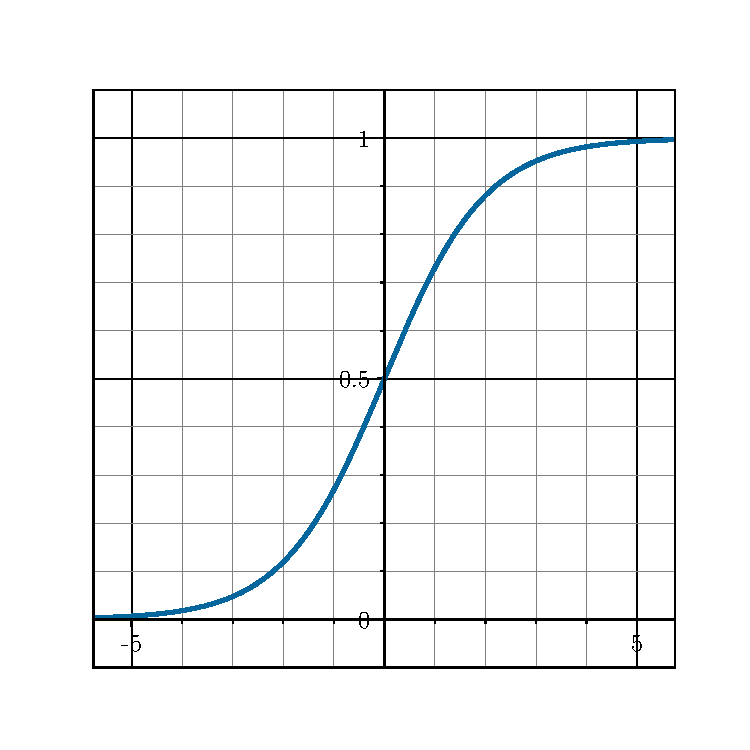
\includegraphics[width=0.98\textwidth]{figures/main/ch2-background/sigmoid.pdf}
    \caption{Sigmoid Activation}
  \end{subfigure}
  \hfill
  \begin{subfigure}[b]{0.32\textwidth}
    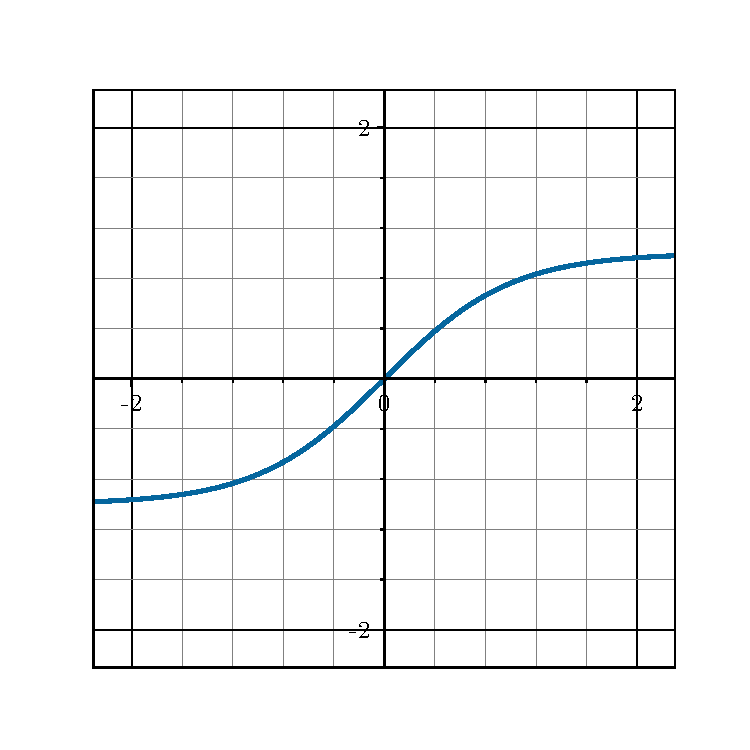
\includegraphics[width=0.98\textwidth]{figures/main/ch2-background/tanh.pdf}
    \caption{Tanh Activation}
  \end{subfigure}
  \hfill
  \begin{subfigure}[b]{0.32\textwidth}
    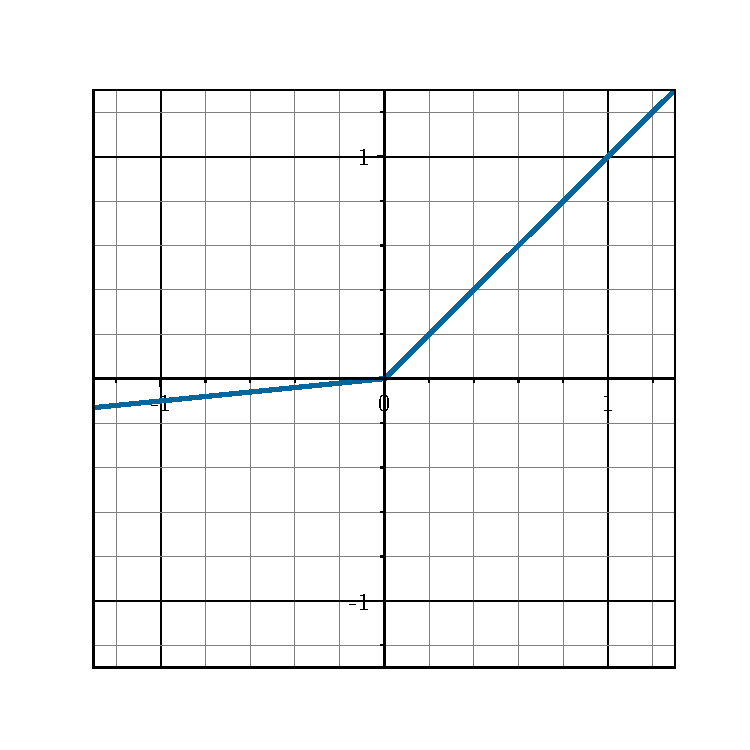
\includegraphics[width=0.98\textwidth]{figures/main/ch2-background/relu.pdf}
    \caption{Leaky-ReLU Activation}
  \end{subfigure}
  \caption{Graphical representation of three common activation functions}
  \label{figure:ch2-activation_functions}
\end{figure}


Choosing the right activation function has been an active area of research. 
Hereafter, we present three common activation functions used by practitioners.
\begin{itemize}
  \item \textbf{Sigmoid activation} \cite{han1995influence}
    \begin{equation*}
      \act(x) = \frac{1}{1+e^{-x}} 
    \end{equation*}
    The sigmoid activation function is one of the first continuous non-linear functions to be used in the context of neural networks.
		It takes a real value as input and outputs another value between 0 and 1.
  \item \textbf{Hyperbolic Tangent activation} \cite{karlik2011performance}
    \begin{equation*}
      \act(x) = \frac{e^x - e^{-x}}{e^x + e^{-x}}
    \end{equation*}
    The hyperbolic tangent activation function is similar to the sigmoid activation function but instead of returning between 0 and 1, the function returns values between -1 and 1.     
  \item \textbf{Leaky Rectified Linear activation (Leaky-ReLU)} \cite{maas2013rectifier}
    \begin{equation*}
      \act(x) = \max(\alpha, x)
    \end{equation*}
    More recently, the ReLU~\cite{nair2010rectified} ($\alpha = 0$) and Leaky-ReLU~\cite{maas2013rectifier} ($\alpha > 0$) activation functions were proposed.
    The parameter $\alpha$ characterizes the slope on $\Rbb_-$.
    These functions have the advantages to avoid the vanishing gradient problem and are less computationally expensive than tanh and sigmoid because it involves simpler mathematical operations.
\end{itemize}

\noindent
\Cref{figure:ch2-activation_functions} presents the graphical representation of the activation functions presented above.
In this thesis, we will use the Leaky-ReLU function with different $\alpha$ when we train deep neural networks.
We simplify the notation $\nn^\act_\weights$ with $\nn_\weights$.




% From $\mathcal{N}$, we can easily build a deep ReLU network $\mathcal{N'}$ of width exactly $n+3$, such that $\forall x \in [0,1]^{n+3}$, $\left|f(\xvec_{1} \ldots \xvec_{n}) - \left(\mathcal{N}'\left(\xvec\right)\right)_{1}\right| < \epsilon$. Thanks to \Cref{lemma:dcnn_approx_neural_network}, this last network can be approximated arbitrarily well by a DCNN of width $n+3$.
%
% \begin{theorem}
%   Let $\Xset \subset \Rbb^{w_{(1)}}$.
%   For any continuous function $f: \Xset \rightarrow \Rbb^{w^{(\depth)}}$, then there exists a  
%
%   Let $\Xset \subset \Rbb^{w_{(1)}}$ and let $f: \Rbb^{w^{(1)}} \rightarrow \Rbb^{w^{(\depth)}}$ be a continuous function.
%   Then, there exists a neural networks parameterized by $\weights$ with an input dimension $w^{(1)}$, an arbitrary depth $\depth$, and $\relu$ activation such that:
%   \begin{equation}
%     \norm{f(\xvec) - \nn(\xvec)} \leq \epsilon
%   \end{equation}
%   \label{theorem:ch2-universal_approximation_theorem}
% \end{theorem}
%


% \citet{cybenko1989approximation} have shown that shallow neural networks with sigmoid activation can \emph{theoretically} approximate any decision boundary.
%
% The arbitrary depth case was also studied by number of authors, such as Zhou Lu et al in 2017,[11] 
% \cite{lu2017expressive}
%
% Boris Hanin and Mark Sellke in 2018,[12] 
% \cite{hanin2017universal}





% %%%%%%%%%%%%%%%%%%%%%%%%%%%%%%%%%%%%%%%%%%%%%%%%%%%%%%%%%%%%%%%%%%%%%%%%%%%%%%%
% \subsection{Adversarial Attacks \& Robustness of Neural Networks}
% \label{subsection:ch2-preliminaries_on_adversarial_attacks}
% %%%%%%%%%%%%%%%%%%%%%%%%%%%%%%%%%%%%%%%%%%%%%%%%%%%%%%%%%%%%%%%%%%%%%%%%%%%%%%%

%%%%%%%%%%%%%%%%%%%%%%%%%%%%%%%%%%%%%%%%%%%%%%%%%%%%%%%%%%%%%%%%%%%%%%%%%%%%%%%
\subsection{Recent Results on the Theory of Neural Networks}
\label{subsection:ch2-recent_results_on_the_theory_of_neural_networks}
%%%%%%%%%%%%%%%%%%%%%%%%%%%%%%%%%%%%%%%%%%%%%%%%%%%%%%%%%%%%%%%%%%%%%%%%%%%%%%%


As seen in the introduction (\Cref{chapter:ch1-introduction}), deep neural networks achieve state-of-the-art performances in a variety of domains such as natural language processing~\cite{radford2018Language}, image recognition~\cite{he2016deep} and speech recognition~\cite{hinton2012deep}.
However, it has been shown that such neural networks are vulnerable to \emph{adversarial examples}, \ie, imperceptible variations of the natural examples, crafted to deliberately mislead the models~\cite{globerson2006nightmare,biggio2013evasion,szegedy2013intriguing}.
Because it is difficult to characterize the space of visually imperceptible variations of a natural image, existing adversarial attacks use $\ell_p$ norms as surrogate measures.
We can formally define an adversarial example as follows:
\begin{definition}[Adversarial Pertubation]
  Given a dataset $\mathcal{S} = \Xset \times \Yset$, a pair $(\xvec, y) \in \mathcal{S}$ and a trained neural network $\nn_\weights$ on $\mathcal{S}$ such that $\argmax_{i \in [0,k-1]} \{ \nn_\weights(\xvec)_i \} = y$, let $\adv \in \Xset$ be an adversarial perturbation such that:
  \begin{align}
    &\argmax_{i \in [0,k-1]} \{ \nn_\weights (\xvec + \adv)_i \} \neq y \\
    \st\ &\norm{\adv}_p \leq \epsilon \notag
  \end{align}
  where $\epsilon$ is a small value defined by the attacker. 
\end{definition}

%%%%%%%%%%%%%%%%%%%%%%%%%%%%%%%%%%%%%%%%%%%%%%%%%%%%%%%%%%%%%%%%%%%%%%%%%%%%%%%
\subsubsection{Implementing Adversarial Attacks}
\label{subsubsection:ch2-adversarial_attacks}
%%%%%%%%%%%%%%%%%%%%%%%%%%%%%%%%%%%%%%%%%%%%%%%%%%%%%%%%%%%%%%%%%%%%%%%%%%%%%%%

Since the discovery of adversarial perturbations, a variety of procedures, \aka \emph{adversarial attacks}, have been developed to generate adversarial examples.
% for example FGSM \cite{goodfellow2014explaining}, PGD \cite{madry2018towards} and C\&W \cite{carlini2017towards}, to mention the most popular ones.
FGSM \cite{goodfellow2014explaining}, PGD \cite{madry2018towards} and \cite{carlini2017towards} to name a few, are the most popular ones.

To find the best perturbation $\adv$, existing attacks can adopt one of the two following strategies:
% \begin{itemize}
%   \item \textbf{Loss maximization}: maximizing the loss $L(\nn_\weights(\xvec + \adv), y)$ under some constraint on $\norm{\adv}_p$ with $p \in \{0, \dots, \infty\}$.;
%   \item \textbf{Perturbation minimization}: minimizing $\norm{\adv}_p$ under some constraint on the loss $L(\nn_\weights(\xvec + \adv), y)$.
% \end{itemize}

\paragraph{Loss maximization.}
In this scenario, the procedure maximizes the loss objective function $L(\nn_\weights(\xvec + \adv), y)$, under the constraint that the $\lp$ norm of the perturbation remains bounded by some value $\epsilon$, as follows:
\begin{equation} \label{equation:ch2-lossmax}
  \argmax_{\adv:\norm{\adv}_p \leq \epsilon} L(\nn_\weights(\xvec + \adv), y) \enspace.
\end{equation}
The typical value of $\epsilon$ depends on the norm $\norm{\ \cdot\ }_p$ considered in the problem setting.
% In order to compare $\linf$ and $\ltwo$ attacks of similar strength, we choose values of $\epsilon_\infty$ and $\epsilon_2$ (for $\linf$ and $\ltwo$ norms respectively) which result in $\linf$ and $\ltwo$ balls of equivalent volumes.
% For the particular case of CIFAR-10, this would lead us to choose $\epsilon_\infty = 0.03$ and $\epsilon_2 = 0.8$ which correspond to the maximum values chosen empirically to avoid the generation of visually detectable perturbations. 
The current state-of-the-art method to solve \Cref{equation:ch2-lossmax} is based on a projected gradient descent (PGD)~\cite{madry2018towards} of radius~$\epsilon$.
Given a budget $\epsilon$, it recursively computes
\begin{equation} \label{equation:ch2-projectionPGD}
  \xvec^{(t+1)} = \prod_{\mathcal{B}_p(\xvec,\epsilon)}\left(\xvec^{(t)}
    + \alpha \argmax_{\adv: \norm{\adv}_p \leq 1} \nabla_\xvec L\left( \nn_\weights \left(\xvec^{(t)} + \adv \right), y \right)
\right)
\end{equation}
where $\mathcal{B}_p(\xvec,\epsilon) = \{ \xvec + \adv:\norm{\adv}_p \leq \epsilon\}$, $\alpha$ is a gradient step size, and $\prod_S$ is the projection operator on $S$.
The PGD attack is currently used in the literature with $p=2$ and $p=\infty$.
The attack with the norm $p=\infty$ is state-of-the-art for the loss maximization problem. 

\paragraph{Perturbation minimization.}
This type of procedure searches for the perturbation with the minimal $\lp$ norm, under the constraint that $L(\nn_\weights(\xvec + \adv), y)$ is bigger than a given bound $c$:
\begin{align}
  &\argmin_{\adv} \norm{\adv}_p \label{equation:ch2-normmin} \\
  \st\ &L(\nn_\weights(\xvec + \adv), y) \geq c \notag
\end{align}
The value of $c$ is typically chosen depending on the loss function $L$.
For example, if $L$ is the $0-1$ loss, any $c > 0$ is acceptable.
\Cref{equation:ch2-normmin} has been tackled by~\citet{carlini2017towards}, leading to the following method, denoted C\&W attack in the rest of the chapter.
It aims at solving the following Lagrangian relaxation of \Cref{equation:ch2-normmin}:
\begin{equation}
  \argmin_{\adv} \norm{\adv}_p + \lambda g(\xvec+\adv)
\end{equation}
where $g(\xvec + \adv)<0$ if and only if $L(\nn_\weights(\xvec + \adv),y) \geq c$. 
The authors use a change of variable $\adv = \tanh(\wvec) - \xvec$ to ensure that $\xvec + \adv \in \Xset$, a binary search to optimize the constant $c$, and Adam or SGD to compute an approximated solution.
The C\&W attack is currently used in the literature with $p \in \{1, 2, \infty \}$ and is state-of-the-art with $p=2$ for the perturbation minimization problem.
% This attack with the norm $p=2$ is state-of-the-art for the perturbation minimization problem. 
% The C\&W attack is well defined both for $p=2$, and $p=\infty$, but there is a clear empirical gap of efficiency in favor of the $\ltwo$ attack.


% For example, \citet{goodfellow2014explaining} use the $\linf$ norm to measure the distance between the original image and the adversarial image whereas \citet{carlini2017towards} use the $\ltwo$ norm.
% When the input dimension is low, the choice of the norm is of little importance because the $\linf$ and $\ltwo$ balls overlap by a large margin, and the adversarial examples lie in the same space.
% For typical image datasets with large dimensionality, the two balls are mostly disjoint.
% As a consequence, the $\linf$ and the $\ltwo$ adversarial examples lie in different areas of the space, and it explains why $\linf$ defense mechanisms perform poorly against $\ltwo$ attacks and vice versa. 



%%%%%%%%%%%%%%%%%%%%%%%%%%%%%%%%%%%%%%%%%%%%%%%%%%%%%%%%%%%%%%%%%%%%%%%%%%%%%%%
\subsubsection{Defending against Adversarial Attacks}
\label{subsubsection:ch2-defending_against_adversarial_attacks}
%%%%%%%%%%%%%%%%%%%%%%%%%%%%%%%%%%%%%%%%%%%%%%%%%%%%%%%%%%%%%%%%%%%%%%%%%%%%%%%

Given the important security risks that adversarial attacks pose, it is important to design defenses to protect neural networks against these kinds of attacks.
Adversarial Training was introduced by~\citet{goodfellow2014explaining} and later improved by~\citet{madry2018towards} as a first defense mechanism to train robust neural networks.
It consists in augmenting training batches with adversarial examples generated during the training procedure.
The structural risk minimization paradigm is thus replaced by the following $\min$ $\max$ problem, where the classifier tries to minimize the expected loss under the maximum perturbation of its input:
\begin{equation}
  \argmin_\weights \argmax_{\adv: \norm{\adv} \leq \epsilon} \frac{1}{|\mathcal{S}|} \sum_{(\xvec, y) \in \mathcal{S}} L\left( \nn_\weights \left(\xvec + \adv \right), y \right) + \lambda \sum_{(\Wmat, \bvec) \in \weights} \left( \norm{\Wmat}_\mathrm{F} + \norm{\bvec}_\mathrm{2} \right)
\end{equation}
% In the case where $p = \infty$, this technique offers good robustness against $\linf$ attacks \cite{athalye2018obfuscated}.
Although adversarial training lacks formal guarantees, it is one of the few techniques that proves to be empirically very effective.


% Despite some recent work providing great insights \cite{sinha2017certifying,zhang2019theoretically}, there is no worst case lower bound yet on the accuracy under attack of this method.




% \%\%\%
%
% \cite{goodfellow2014explaining} have proposed \textbf{Adversarial Training} which follows \textbf{ERM} training over adversarially-perturbed samples
%
%
% \%\%\%

% Another important technique to defend against adversarial examples is to use \emph{noise injection} techniques.  
% In contrast with adversarial Training, noise injection mechanisms are usually deployed after training.


% In a nutshell, it works as follows.
% At inference time, given a unlabeled sample $x$, the network outputs
% \begin{equation}
%   \tilde{f}_\theta(\xvec) \triangleq f_\theta(\xvec + \eta) \ \ \ (\text{instead of  } f_\theta(\xvec)) 
% \end{equation}
% where $\eta$ is a random variable on $\mathbb{R}^d$.
% Even though, Noise Injection is often less efficient than Adversarial Training in practice (see \eg, \Cref{table:764774}), it benefits from strong theoretical background.
% In particular, recent works \cite{lecuyer2018certified,li2019certified}, followed by~\citet{cohen2019certified,pinot2019theoretical} demonstrated that noise injection from a Gaussian distribution can give provable defense against $\ltwo$ adversarial attacks.
% In this work, besides the classical Gaussian noises already investigated in previous works, we evaluate the efficiency of Uniform distributions to defend against $\ltwo$ adversarial examples. 





%%%%%%%%%%%%%%%%%%%%%%%%%%%%%%%%%%%%%%%%%%%%%%%%%%%%%%%%%%%%%%%%%%%%%%%%%%%%%%%%
\section{Summary of the Chapter}
\label{section:ch2-summary_of_the_background}
%%%%%%%%%%%%%%%%%%%%%%%%%%%%%%%%%%%%%%%%%%%%%%%%%%%%%%%%%%%%%%%%%%%%%%%%%%%%%%%%

As explained in the Introduction (\Cref{chapter:ch1-introduction}), our contributions lie at the intersection between neural networks and structured matrices.
In this chapter, we have reviewed the necessary concepts to present our contributions and some related work.

First, \Cref{section:ch2-a_primer_on_circulant_and_toeplitz_matrices} introduces circulant and Toeplitz matrices which are the main mathematical objects used in this thesis.
Circulant and Toeplitz matrices are structured matrices in which each descending diagonal, from left to right, is constant.
These structured matrices are the building blocks of our contribution on compact neural networks (\Cref{chapter:ch4-diagonal_circulant_neural_network}) and enable fast approximation of the Lipschitz constant of convolutional layers leading to a new regularization scheme (\Cref{chapter:ch5-lipschitz_bound}).

Finally, in \Cref{subsection:ch2-introduction_on_supervised_learning}, we gave a quick overview of the concept of supervised learning, which presents the mathematical tools for optimizing a parameterized function in order to map an input to an output based on a series of input-output pairs.
Although the statistical learning framework considers generic hypothesis space, in this work we use a class of functions called neural networks presented in \Cref{subsection:ch2-preliminaries_on_neural_networks}.
We also presented, in \Cref{subsection:ch2-adversarial_attacks_robustness_of_neural_networks}, the concept of adversarial attacks and robustness of neural networks.
We showed how a neural network can be sensitive to small perturbations to its input and thus vulnerable to adversarial examples.
Reducing the sensitivity and therefore increasing the robustness of neural networks is the central theme of our second contribution presented in \Cref{chapter:ch5-lipschitz_bound}.
Finally, in \Cref{subsection:ch2-recent_results_on_the_theory_of_neural_networks}, we have presented some recent results on the theory of neural networks.
These results give us important insights on how neural networks generalize and a theoretical justification of the regularization scheme that we propose in \Cref{chapter:ch5-lipschitz_bound}.





